% Document uses 12 pt font
% 1 in margins
% Contains a relative path for images

% CHANGES 
% 1. Requirements to modules Traceability matrix (requirements vs modules) 
        % - completed but needs to be verified
        
% 2. Unexpected Event Handling goes in the component descriptions
% 3. Hardware Schematics 
        %--> put under vehicle hardware section 
        
        
% 4. Traceability matrix for possible changes (changes vs modules) 
         % - completed but needs to be verified
         
% 5. Update Modules 
% 6. Assumptions & constraints (goes in Intro) 
    % - completed but needs to be verified
    
% 7. Check system components inputs and outputs are correct


%%%%%%%%%%%%%%%%%%%%%%%%%%%%%%%%%%%%%%%%%%%%%
\documentclass [10pt]{article}

% page geometry 
\usepackage[margin=1in]{geometry}


% ----------  PACKAGES START ------------ %
% Math Packages
\usepackage{amsmath}
\usepackage{mathtools}

% Table cell color package and highlighting
\usepackage[table]{xcolor}
\usepackage{color,soul}

% VIC title package
\usepackage{cabin}
\usepackage[T1]{fontenc}

% default font package
%\usepackage{times}
\usepackage{helvet}
%\renewcommand{\familydefault}{\sfdefault}

% ---------- End Font Packages -------------- %

\usepackage{listings}


\definecolor{dkgreen}{rgb}{0,0.6,0}
\definecolor{gray}{rgb}{0.5,0.5,0.5}
\definecolor{mauve}{rgb}{0.58,0,0.82}

\lstset{frame=tb,
  language=C++,
  aboveskip=3mm,
  belowskip=3mm,
  showstringspaces=false,
  columns=flexible,
  basicstyle={\small\ttfamily},
  numbers=none,
  numberstyle=\tiny\color{gray},
  keywordstyle=\color{blue},
  commentstyle=\color{dkgreen},
  stringstyle=\color{mauve},
  breaklines=true,
  breakatwhitespace=true,
  tabsize=3
}

% Title Packages
\usepackage{titlesec}
\usepackage{titletoc}

% Image Package
\usepackage{graphicx}

% Table Packages
\usepackage{longtable}
\usepackage{multirow}
\usepackage{multicol}
\usepackage{multirow}
\usepackage{array}
\renewcommand{\arraystretch}{1.2}% Spread rows out evenly in table
\setlength{\LTpre}{0.5pt} % Reduces white space around tables (top)
%\setlength{\LTpost}{0pt} % Reduces white space around tables (bottom)

% Color Packages
\usepackage{color}   
\definecolor{sectionC}{rgb}{0.016,0.227,.365}
\definecolor{subsectionC}{rgb}{.87,0.87,.87}
\definecolor{subsubsectionC}{rgb}{.94,.93,.90}
\definecolor{tableCell}{rgb}{.96,.95,.90}


% List package
\usepackage{enumitem}
\setenumerate{itemsep=0pt, itemindent=0in,leftmargin=0.5in}


% Paragraph parameter

\setlength{\parindent}{0pt}


% ------------- Creates a linked Table of Contents  Start --------------- %
\usepackage{hyperref}
\hypersetup{
colorlinks=true, %set true if you want colored links
linktoc=all,     %set to all if you want both sections and subsections linked
linkcolor=black,}  %choose some color if you want links to stand out

% ------------- Creates a click-able Table of Contents  End--------------- %

% ---------- PACKAGES END ------------ %


% ------------ BEGIN LANDSCAPE MODE ----------------%
\usepackage{pdflscape}
% ------------ END LANDSCAPE MODE ----------------%





% -------- SECTION AND SUBSECTION FORMATING START -------- % 
% starts the 
%\setcounter{section}{1}


\titleformat{\section} % Section
{\normalfont \fontsize{14}{14} \bfseries}{}{0em}{\colorsection}

% Makes a background color
\newcommand{\colorsection}[1]{%
  \colorbox{sectionC}{\parbox{\dimexpr\textwidth-1\fboxsep}{\color{white}\Large\thesection\ \hspace{1mm} #1}}}

% Makes a background color
\titleformat{\subsection} % Subsection
{\normalfont \fontsize{12}{12}  \bfseries}{}{0em}{\colorsubsection }

\newcommand{\colorsubsection}[1]{%
  \colorbox{subsectionC}{\parbox{\dimexpr \textwidth -1\fboxsep}{\large\thesubsection\ #1}}}


% Makes a background color
\titleformat{\subsubsection} % Subsubsection
{\normalfont \fontsize{12}{12} \bfseries}{}{0em}{\colorsubsubsection}

\newcommand{\colorsubsubsection}[1]{%
  \colorbox{subsubsectionC}{\parbox{\dimexpr\textwidth-1\fboxsep}{\thesubsubsection\ #1}}}

% -------- SECTION AND SUBSECTION FORMATING END -------- % 
\usepackage{lipsum}


% -----  IMAGE PATH START -----%
% Relative Image Path
\graphicspath {figures/}
% -----  IMAGE PATH END -----%

% ------ PARAGRAPH FORMAT START ----%
%\setlength{\parskip}{.2em}% Sets the space between new paragraph items 
\setlength{\parindent}{0em} % paragraph indent
% ------ PARAGRAPH FORMAT END ----%




%------------------------------TOC FORMAT START --------------------------------%
\usepackage{tocloft}



% Section indentations
\cftsetindents{section}{0em}{1.5em}
\cftsetindents{subsection}{1em}{2em}
\cftsetindents{subsubsection}{2em}{3em}

% Toc title size
\renewcommand\cfttoctitlefont{\Large\bfseries}
\renewcommand*\contentsname{Table of Contents}

\newcommand{\carSpeed}{1.4\ m/s}
\newcommand{\intersectionLength}{0.6\ m}


% Removes bold headings from toc
%\renewcommand{\cftsecfont}{\normalfont}

% Removes bold heading page numbers from toc
\renewcommand{\cftsecpagefont}{\normalfont}

% add dots after headings
%\renewcommand{\cftsecleader}{\cftdotfill{\cftdotsep}} 


% number of section headings we want to see in toc
\setcounter{tocdepth}{2}

% Spaceing before headings in toc
\setlength{\cftbeforesecskip}{6pt}

% ------------------------------TOC FORMAT END --------------------------------%


% ------------------- START ROTATE FOOTER ---------------------------%
\usepackage{everypage}


\newcommand{\Lpagenumber}{\ifdim\textwidth=\linewidth\else\bgroup
  \dimendef\margin=0
  \ifodd\value{page}\margin=\oddsidemargin
  \else\margin=\evensidemargin
  \fi
  \raisebox{\dimexpr -\topmargin-\headheight-\headsep-.8\linewidth}[0pt][0pt]{%
    \rlap{\hspace{\dimexpr \margin+\textheight}%
    \llap{\rotatebox{0}{Page \textbf{\thepage}\ of \textbf{\pageref{LastPage}}}}}}%
\egroup\fi}
\AddEverypageHook{\Lpagenumber}%

% ------------------- END ROTATE FOOTER ---------------------------%



% ------------------- START HEADER AND FOOTER ---------------------------%
\usepackage{fancyhdr}

% Helps with the n of total n pages
\usepackage{lastpage}

\pagestyle{fancy}

% Header
\lhead{System Design }
\rhead{Revision: 1}
\fancyhead[LE,CO]{VIC - Group 6}

% Removes line under the header 
\renewcommand{\headrulewidth}{0pt}
\setlength{\headsep}{.2in}

% Footer 

% Set the right side of the footer to be the page number
\fancyfoot[R]{Page \textbf{\thepage}\ of \textbf{\pageref{LastPage}}}
\fancyfoot[C]{}

% ------------------- END HEADER AND FOOTER ---------------------------%






% -------------- DOCUMENT START ---------------%
\begin{document}

% --------- TITLE PAGE START ------- %
\begin {center} 

\thispagestyle{empty}
\vspace*{5cm}

% Logo Insertion
\begin {figure}[h!]
\centering
\hspace{-10mm}
\includegraphics [scale = .5, trim={.4cm 0 .8cm 0},clip] {figures/vic_logo.png}
\end {figure}

{\fontfamily{\cabinfamily}\selectfont
\Huge{Vehicle Intersection Control} }

\vspace{1 cm}
{\Large\textbf{\textsc{McMaster University}}\\}  \vspace {1cm}
{\Large System Design\\ \vspace {0.4 cm} SE 4G06}  \vspace {1cm}

{\large \textsc{Group 6} \\} \vspace{1cm}

\begin{tabular}{ l c  l}
Alex Jackson &-& 1302526\\
Jean Lucas Ferreira &-& 1152120 \\
Justin Kapinski &-& 1305257\\
Mathew Hobers &-& 1228607\\
Radhika Sharma &-& 1150430\\
Zachary Bazen &-& 1200979
\end{tabular}




\end{center}

% --------- TITLE PAGE END------- %

\pagebreak

% Inserting table of contents and table of figures 

\tableofcontents
\listoftables
\listoffigures



\pagebreak

% -----------  REVISION HISTORY START ----------- %

%\section*{Revisions}

\section{Revisions}
\begin{longtable}{| p{.2\textwidth } | p{.23\textwidth } | p{.2\textwidth } | p{.27\textwidth } |} \caption{VIC Table of Revisions}  \\

\hline 
\centering \textbf{Date} & 
\multicolumn{1}{c}{\textbf {Revision Number}} &
\multicolumn{1}{|c}{\textbf {Authors}} & 
\multicolumn{1}{|c|}{\textbf {Comments}} \\ \hline


\multicolumn{1}{|c|}{\multirow{1}{*}{\centering March 25, 2017}}  & 
\multicolumn{1}{c|}{\multirow{1}{*}{Revision 1}} &
\begin{minipage}{.21\columnwidth}
\vspace{1mm}
    Alex Jackson \newline
    Jean Lucas Ferreira \newline
    Justin Kapinski\newline
    Mathew Hobers\newline
    Radhika Sharma\newline
    Zachary Bazen     \vspace{1mm}
\end{minipage}&
\begin{minipage} {.27\columnwidth}
    \begin{enumerate}[label = - , leftmargin=0.11in]
        \itemsep -.5em
        \item Updated system component information
        \item Added unexpected even handling 
        \item Updated system component information
        \item Updated MIS and MID information
        \item Added circuit diagrams \vspace{1.5mm}
    \end{enumerate}
\end{minipage}\\ \hline 


\multicolumn{1}{|c|}{\multirow{1}{*}{\centering March 24, 2017}}  & 
\multicolumn{1}{c|}{\multirow{1}{*}{Revision 1}} &
\begin{minipage}{.21\columnwidth}
\vspace{1mm}
    Alex Jackson \newline
    Jean Lucas Ferreira \newline
    Justin Kapinski\newline
    Mathew Hobers\newline
    Radhika Sharma\newline
    Zachary Bazen     \vspace{1mm}
\end{minipage}&
\begin{minipage} {.27\columnwidth}
    \begin{enumerate}[label = - , leftmargin=0.11in]
        \itemsep -.5em
        \item Updated module numbering
        \item Added module to requirement traceability matrix
        \item Added module change likelihood and ways to change \vspace{1mm}
    \end{enumerate}
\end{minipage}\\ \hline 

\multicolumn{1}{|c|}{\multirow{1}{*}{\centering March 20, 2017}}  & 
\multicolumn{1}{c|}{\multirow{1}{*}{Revision 1}} &
\begin{minipage}{.21\columnwidth}
\vspace{1mm}
    Alex Jackson \newline
    Jean Lucas Ferreira \newline
    Justin Kapinski\newline
    Mathew Hobers\newline
    Radhika Sharma\newline
    Zachary Bazen     \vspace{1mm}
\end{minipage}&
\begin{minipage} {.27\columnwidth}
    \begin{enumerate}[label = - , leftmargin=0.11in]
        \itemsep -.5em
        \item Combined phase 1 documents and phase 2 documents
        \item Split MIS and MID into two distinct sections\vspace{1mm}
    \end{enumerate}
\end{minipage}\\ \hline 


\multicolumn{1}{|c|}{\multirow{5}{*}{\centering January 25, 2017} } & 
 \multicolumn{1}{c|}{\multirow{5}{*}{Revision 0}}& 
{Alex Jackson \newline
Jean Lucas Ferreira \newline
Justin Kapinski\newline
Mathew Hobers\newline
Radhika Sharma\newline
Zachary Bazen}
&
% \begin{minipage} {.27 \columnwidth}
%     \begin{enumerate}[label = - , leftmargin=0.11in]
%         \itemsep -.5em
%         \item  System design phase 2\vspace{1mm}
%     \end{enumerate}
% \end{minipage}  \\ 
\multicolumn{1}{|c|}{\multirow{5}{*}{\centering - System design phase 2}} \\\hline



\multicolumn{1}{|c|}{\multirow{5}{*}{\centering December 21, 2016}}  & 
 \multicolumn{1}{c|}{\multirow{5}{*}{Revision 0}}& 
{Alex Jackson \newline
Jean Lucas Ferreira \newline
Justin Kapinski\newline
Mathew Hobers\newline
Radhika Sharma\newline
Zachary Bazen}
&
\multicolumn{1}{|c|}{\multirow{5}{*}{\centering - System design phase 1}} \\
% \begin{minipage} {.27 \columnwidth}
%     \begin{enumerate}[label = - , leftmargin=0.11in]
%         \itemsep -.5em
%         \item  System design phase 1\vspace{1mm}
%     \end{enumerate}
% \end{minipage}  \\ 
\hline 

 \end{longtable}
% % -----------  REVISION HISTORY END ----------- %
 \pagebreak

%---------------------------- PROJECT DRIVERS ------------------------%
% heading in document

% -------------- START INTRODUCTION ---------------- %
\section {Introduction}

\subsection{Document Purpose}




Vehicle Intersection Controller (VIC) is a system that allows autonomous cars to proceed through four way stop intersections when the vehicles arrive. The purpose of this document is to provide a comprehensive system overview of the VIC  system. In addition, it is intended to provide comprehensive subsystem details that will allow the system to be implemented.  


\subsection{System Scope}
VIC will focus on solving the aforementioned problem on a controlled, indoor track.  Autonomous vehicles, using a $\frac{1}{10}$ scale, will be used to simulate real world autonomous cars. To prevent damage of hardware, the autonomous vehicles will be able to detect obstacles. VIC will ignore situations involving non-autonomous cars. 




\subsection{Document Overview and Intended Audience}
This document contains multiple sections that will provide information on: system assumptions and constraints,  overall system information, descriptions and diagrams of system components, detailed module interface and design information along with sequence diagrams. \\

The system overview contains a natural language description of the VIC system and appropriate context diagrams. In the system components section a high level description is given of the inputs and outputs of the VIC system. This is followed by a module guide. \\

The module guide provides an overview of all the system modules and a natural language description of each module. Each module description includes information on intended behaviour, inputs, outputs, initialization and timing constraints. In addition, a traceability matrix to requirements is included for all modules and the likelihood of change for each module.  \\

This is followed by the Module Interface Specification and Module Internal Design sections. These sections provide detailed information on VIC module interfaces and internal designs. The final section contains system sequence diagrams. \\


When reading this document it will be helpful to note that there are two main components to VIC. These two components are the intersection component and the vehicle component.  Sections are organized with this division.   \\

The intended audience for this document is Sean Marshall (the engineering team leader at GM) who proposed the problem, Dr. Alan Wassyng and the teaching assistants as supervisors of the project, and ourselves as designers of the system.

% Naming Conventions

\subsection{Acronyms}

\begin{longtable}{ |p{.23\textwidth } p{.725\textwidth }|} \caption{Acronyms} \\ \hline


\textbf{VIC} & Vehicle Intersection Control \\ 

\cellcolor{tableCell}\textbf{IC}  & \cellcolor{tableCell}Intersection Controller \\

\textbf{VC} &Vehicle Controller\\\hline


\end{longtable}

\subsection{Definitions}

\begin{longtable}{ |p{.23\textwidth } p{.725\textwidth }|} \caption{Definitions} \\ \hline


\textbf{VIC} & The entire system including the intersection controller, the vehicles, and their corresponding controllers. \\ 

\rowcolor{tableCell}\textbf{IC}  & The Intersection Controller is the system that tracks the arrival and departure of the vehicles, as well as determining the order in which the vehicles must proceed through the intersection.\\

\textbf{VC} & The Vehicle Controller is the system that will allow the 1/10 scale RC car to follow lanes, maintain a desired speed, steer itself, and send requests to the intersection controller. \\\hline


\end{longtable}

\subsubsection{Naming Conventions}
\begin{longtable}{ |p{.23\textwidth } p{.725\textwidth }|} \caption{Naming Conventions} \\ \hline
\textbf{A\#} & Assumptions \\ 
\rowcolor{tableCell}\textbf{MC\#} & Mandated Constraint \\ 
\textbf{ICM\#} & Intersection Controller Module \\ 

\rowcolor{tableCell}\textbf{VCM\#} & Vehicle Controller Module\\
\textbf{VHM\#}  & Vehicle Hardware Module \\

\rowcolor{tableCell}\textbf{IDC\#} & Intersection design component\\
\textbf{VCD\#}  & Vehicle design component \\\hline

\end{longtable}
\subsubsection{Assumptions}

\begin{longtable}{| p{.2\textwidth } | p{.75\textwidth } | }\hline 
\rowcolor{tableCell}\textbf{A1} & Ideal driving conditions on the track \\ \hline
\textbf{Rationale} & Track is situated indoors \\ \hline 
\end{longtable}

\begin{longtable}{| p{.2\textwidth } | p{.75\textwidth } | }\hline 
\rowcolor{tableCell}\textbf{A2} & Intersection is a four way stop \\ \hline
\textbf{Rationale} &  Different intersection arrangements are beyond the scope of this project \\ \hline
\end{longtable}

\begin{longtable}{| p{.2\textwidth } | p{.75\textwidth } | }\hline 
\rowcolor{tableCell}\textbf{A3} & Only autonomous car will be present on the track \\ \hline
\textbf{Rationale} & Only autonomous vehicles are within the scope of the project \\ \hline
\end{longtable}

\begin{longtable}{| p{.2\textwidth } | p{.75\textwidth } | }\hline 
\rowcolor{tableCell}\textbf{A4} & Vehicles and intersection controller are pre-Bluetooth paired  \\ \hline
\textbf{Rationale} & Speeds up communication by allowing messages to be sent directly to a Bluetooth address without having to first discover them. \\ \hline
\end{longtable}

\begin{longtable}{| p{.2\textwidth } | p{.75\textwidth } | }\hline 
\rowcolor{tableCell}\textbf{A5} & Intersection directions will be labeled by a colour \\ \hline
\textbf{Rationale} & Allows direction information to be acquired without additional hardware\\ \hline 

\end{longtable}


\subsection{Mandated Constraints}


\begin{longtable}{| p{.2\textwidth } | p{.75\textwidth } | }\hline 

\rowcolor{tableCell}\textbf{MC1}& Vehicles must make a complete stop at the intersection before proceeding through\\ \hline 
\textbf{Rationale} & Vehicles must follow the rules of the road\\ \hline 

\end{longtable}


\begin{longtable}{| p{.2\textwidth } | p{.75\textwidth } | }\hline 
\rowcolor{tableCell}\textbf{MC2} & The cars must not turn at the intersection \\ \hline
\textbf{Rationale} & To simplify intersection navigation \\ \hline


\end{longtable}

% \begin{longtable}{| p{.2\textwidth } | p{.75\textwidth } | }\hline 
% \rowcolor{tableCell}\textbf{MC3} & \textbf{The cost of the project must not exceed \$700 dollars} \\ \hline
% \textbf{Rationale} & This is to ensure an off-the-shelf solution can not be purchased. It also ensures the project remains economically feasible. \\ \hline
% \end{longtable}

% \begin{longtable}{| p{.2\textwidth } | p{.75\textwidth } | }\hline 
% \rowcolor{tableCell}\textbf{MC4} & \textbf{The cars must not turn at the intersection} \\ \hline
% \textbf{Rationale} & To simplify intersection navigation \\ \hline


%\end{longtable}


\section{System Overview}


\subsection{Behavior Overview}
     VIC is a system that controls autonomous vehicle traffic flow at an intersection. It consists of two main components, the intersection controller and the autonomous vehicles. These components communicate over Bluetooth communication. \\
      
     The intersection controller uses a camera to  monitor the state of the intersection. Once a vehicle is detected the next intersection state is determined using current autonomous vehicle input and camera data. When the next intersection state is determined, the intersection controller communicates to the appropriate vehicle to proceed. After the vehicle has left, the current intersection state is updated and the next state calculated.   \\


    The autonomous vehicles uses a camera to detect the current position within the lanes of the track, and built-in hardware components such as a servo, and a speed controller to set and maintain desired speed and turning angles. Furthermore, with the help of the camera it will be able to detect when the vehicle is approaching an intersection, or if an obstacle is present in the current path.
    
    
    Obstacle detection ensures the safety of the vehicle and the obstacle itself. Obstacles will detected using the on-board camera and image processing algorithms.  \\
    
    The intersection detection also provides a means for interpreting the current direction the car is approaching from. This feature  will become an important piece of information for determining whether the car should stop at the intersection, or if it can safely proceed. This decision will be determined by the intersection controller. Once the  decision has been finalized, it will signal the vehicle that it may proceed through the intersection.
    

    % This information, along with future destination information will be sent to the intersection controller in order to receive an appropriate proceed signal from that controller. Once the appropriate signal is received the vehicle proceeds through the intersection on its intended course.  
    
    
    
\subsection{Context Diagrams}
\begin{figure} [h!]
	\caption{Intersection Controller Context Diagram} \bigskip
	\centering
	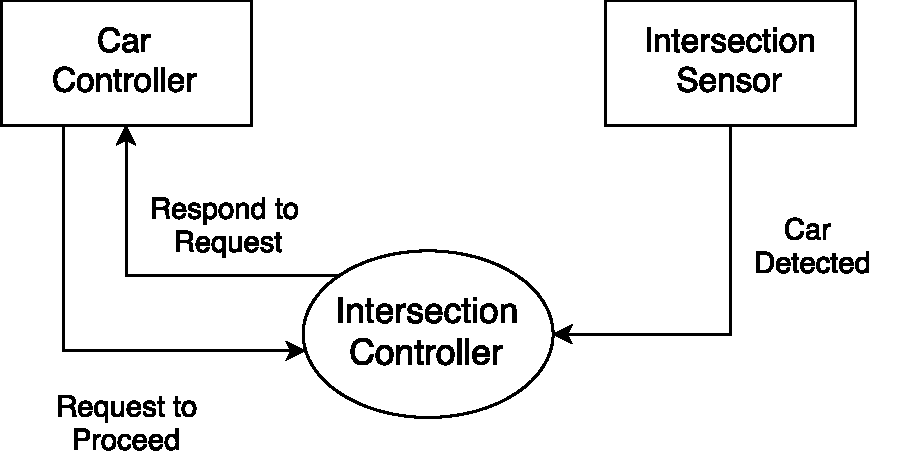
\includegraphics [scale = 0.8] {figures/IC_ContextDiagram.pdf}

\end{figure}
\pagebreak
\begin{figure} [h!]
	\caption{Car Controller Context Diagram} \bigskip
	\centering
	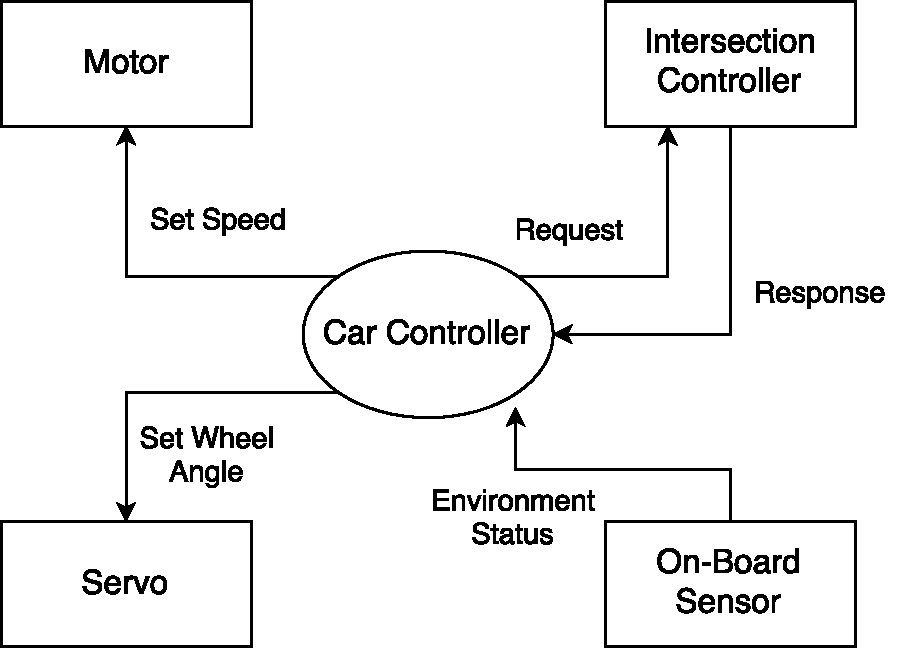
\includegraphics [scale =0.8] {figures/CarCtrl_ContextDiag.pdf}

\end{figure}





%Insert Text or Image Here. 

%-------------- END OVERALL DESIGN DESCRIPTION  ---------------- %




% -------------- START SYSTEM COMPONENTS ---------------- %
\section{System Components}
 


\subsection{System Components Description}

\begin{longtable}{p{.98\textwidth}}
\rowcolor{tableCell}\textbf{IDC.1 - Intersection Design Component} \\
\end{longtable}

\textbf{Description} \\
This component makes uses of Bluetooth communication and a camera that will be controlled by the Intersection Controller. The intersection controller is responsible for gathering intersection state information and vehicle requests. It uses this information to determine the order vehicles should proceed through the intersection.
Once the intersection has been determined to be safe, the system sends a proceed command to the respective vehicle. \\

There are two external inputs to this component. Firstly, a human input, that will allow the initialization of the intersection controller by turning it on. Secondly, a Bluetooth signal, which will occur during run time when a vehicle sends a request ot notify its intent to drive through the intersection.
% comes in with past and intended direction information along information where to send the return command.

% The inputs for this component are human and one Bluetooth signal. The first input initializes the intersection controller. The second input will occur at run time when a vehicle request comes in with past and intended direction information along information where to send the return command.  \\


Upon initialization, the intersection controller will initialize all required modules and  starts the Bluetooth communication.\\

% \textbf{Inputs} \vspace{-2mm}
% \begin{enumerate}[label = - , leftmargin=0.25in]
%         \itemsep -.5em
%         \item vehicle\_request(s)
%         \item video\_capture[x][y]
%     \end{enumerate}



% \textbf{Outputs}\vspace{-2mm}
% \begin{enumerate}[label = - , leftmargin=0.25in]
%         \itemsep -.5em
%         \item car\_signal(s)
%     \end{enumerate}

% \textbf{Timing Constraints}\vspace{-2mm}
% \begin{enumerate}[label = - , leftmargin=0.25in]
%         \itemsep -.5em
%         \item 1 second intersection arrival decision
%         \item 1 second intersection schedule
%         \item $\frac{1}{2}$ second intersection departure decision 
%     \end{enumerate}

% \textbf{Deadline}\vspace{-2mm}
% \begin{enumerate}[label = - , leftmargin=0.25in]
%         \itemsep -.5em
%         \item Decisions must be made before the next intersection arrival poll
%     \end{enumerate}

% \textbf{Initialization} \vspace{-2mm}
% \begin{enumerate}[label = - , leftmargin=0.25in]
%         \itemsep -.5em
%         \item Clear all intersection arrival queues 
%         \item Create a listening socket to receive vehicle requests
%         \item Initialize intersection state and store first frame webcam data 
%     \end{enumerate}
    
% \pagebreak
    
\begin{longtable}{p{.98\textwidth}}
\rowcolor{tableCell}\textbf{VDC.1 - Vehicle Design Component} \\
\end{longtable}








\textbf{Description} \\
This component makes use of a $\frac{1 }{10}$ scale, electric car that will be controlled by the Vehicle Controller. The vehicle controller is responsible for gathering and interpreting vehicle environment information. This information is used to control the vehicles behaviour. %about the vehicle's current position on the track, and interpreting the data in a way that dictates how the vehicle should behave.  
The vehicle will follow the lanes of the track, and stop when an intersection or obstacle is present, by utilizing the servo and speed controller of vehicle. Furthermore, when it begins to approach an intersection, it will send a request to proceed to the intersection controller. Once the intersection controller has approved the request,  the vehicle will continue its path. \\

This component will have two sources of external inputs: one human and one Bluetooth signal. The first input is the human interaction that turns on the vehicle, and initializes the vehicle controller. The second input will occur when the vehicle is operational, and receives a Bluetooth signal from the Intersection Controller with some desired value stating an action that vehicle should take. \\

Upon initialization, the vehicle controller will initialize all required modules, and keep the vehicle in a stopped position until a go-ahead signal is given.

\subsection{System Components Diagram}


\begin{figure} [h!]
	\caption{System Component Diagram - Vehicle Component} \bigskip
	\hspace*{-1.5cm}
	\includegraphics [scale =0.55] {figures/Overall_system_component_diagram.png}

    
\end{figure}

\pagebreak
\begin{figure} [h!]
	\caption{System Component Diagram} \bigskip
	\hspace*{-1.5cm}
	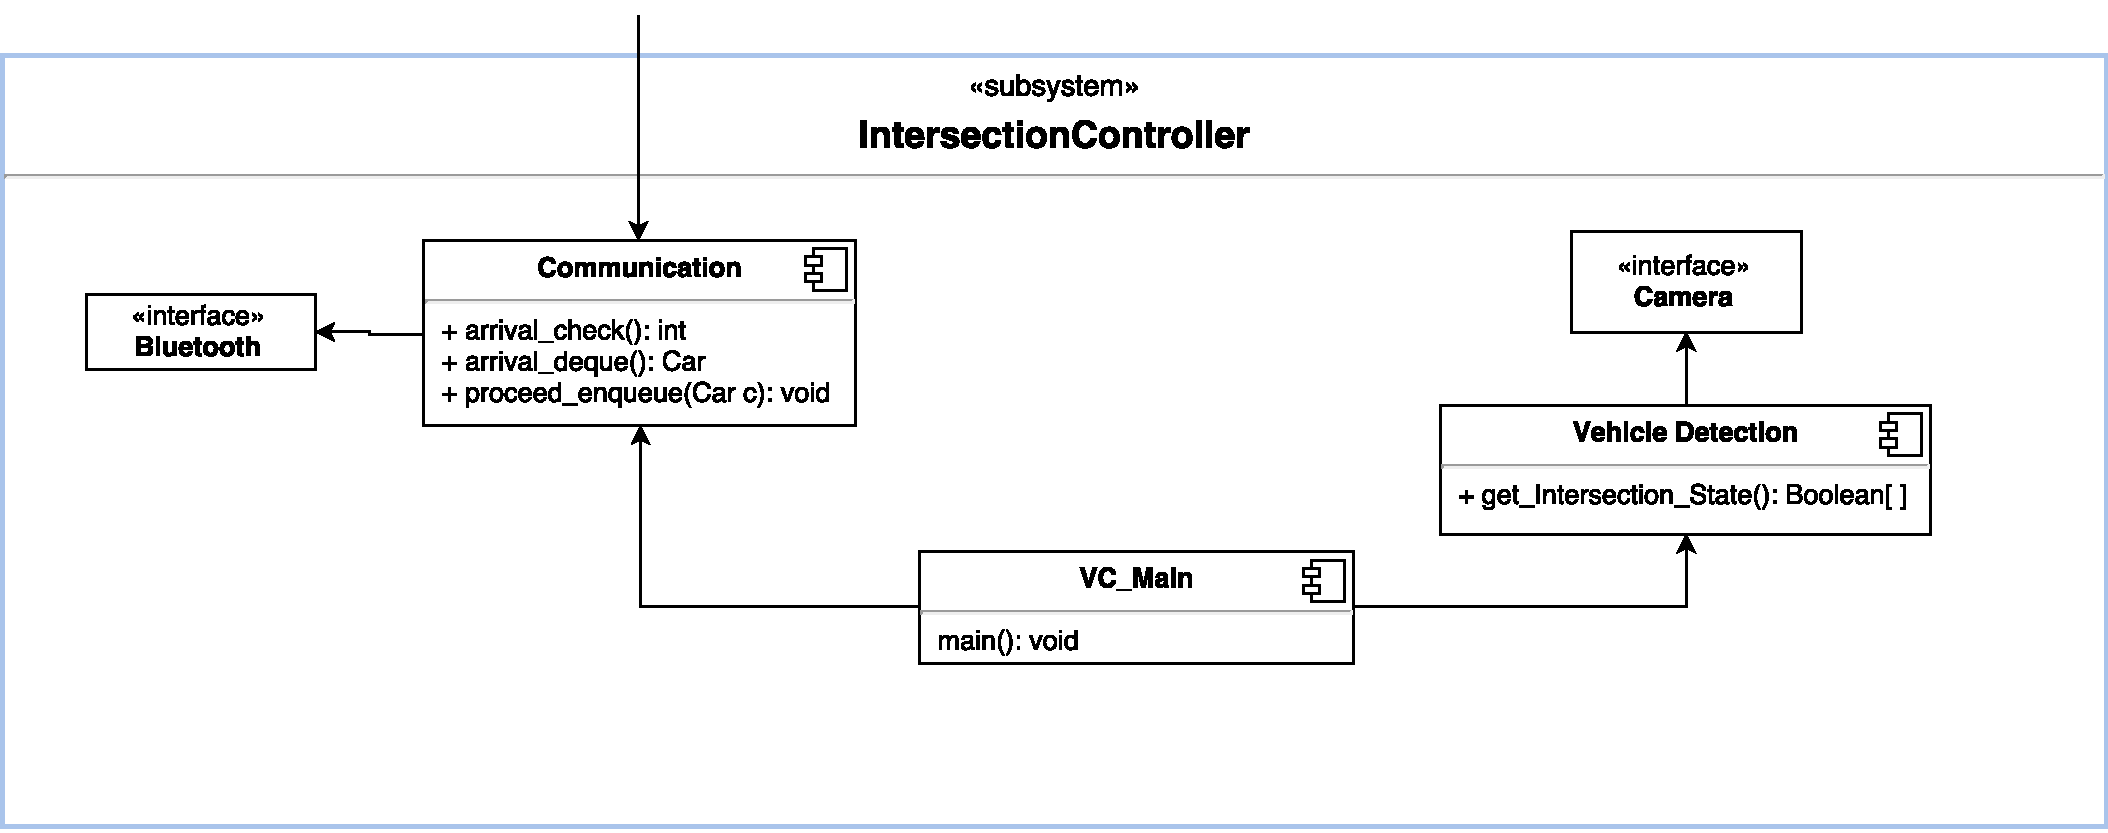
\includegraphics [scale =0.55] {figures/componDiagram2.pdf}

    
\end{figure}



% % removed m_vc_ from in front of each section --> we removed monitored and controlled variable nameing conventions
% \textbf{Inputs} \vspace{-2mm}
% \begin{enumerate}[label = - , leftmargin=0.25in]
%         \itemsep -.5em
%         \item video\_capture[x][y]
%         \item frontDistance
%         \item hallEffect
%         \item carProceedSignal
        
%     \end{enumerate}



% \textbf{Outputs}\vspace{-2mm}
% \begin{enumerate}[label = - , leftmargin=0.25in]
%         \itemsep -.5em
%         \item wheelAngle
%         \item carSpeed
%         \item vehicleBreak
%         \item request\_The\_IC
%     \end{enumerate}

% \textbf{Timing Constraints}\vspace{-2mm}
% \begin{enumerate}[label = - , leftmargin=0.25in]
%         \itemsep -.5em
%         \item Process images for 20 ms
%     \end{enumerate}


% \textbf{Initialization} \vspace{-2mm}
% \begin{enumerate}[label = - , leftmargin=0.25in]
%         \itemsep -.5em 
%         \item Initialize all speed controls to zero
%         \item Initialize wheel angle to zero
%         \item Connect to intersection over Bluetooth communication
%     \end{enumerate}



% -------------- END SYSTEM COMPONENTS  ---------------- %

\section{Module Guide}

\subsection{Module Overview}

% IC modules - hardware and software
\subsubsection{Intersection Controller Modules}

\begin{longtable}{ |p{0.1\textwidth }  | p{0.2\textwidth } |  p{0.3\textwidth } |  p{0.3\textwidth } |}  \hline
    
    \textbf{ID} & \textbf{Name} &  \textbf{Responsibilities} & \textbf{Secrets} \\ \hline
    

    
    \rowcolor{tableCell}ICM.1 & VehicleDetection & Know when a car is within intersection area & Relationship between intersection camera and car \\ \hline
    
    ICM.2  &Communication & Interpret receiving car signals and sending signals to a car & Communication protocol \\ \hline
    
    
        \rowcolor{tableCell}ICM.3 & IC\_Main & Determine order of vehicle progression based in input data & Scheduling algorithm   \\ \hline

\end{longtable}


%  Vehicle Software modules
\subsubsection{Vehicle Controller Software Modules}

\begin{longtable}{ |p{0.1\textwidth }  | p{0.2\textwidth } |  p{0.3\textwidth } |  p{0.3\textwidth } |}  \hline
    
    \textbf{ID} & \textbf{Name} &  \textbf{Responsibilities} & \textbf{Secrets} \\ \hline
    
    \cellcolor{tableCell}VCM.1  &\cellcolor{tableCell}ImageProcessing &\cellcolor{tableCell}Interpret image into environment state &\cellcolor{tableCell}Image processing algorithm  \\ \hline
    
    VCM.2 & VehicleNavigaton & Control the navigation of the car & How the car navigates on the track \\ \hline
    % \cellcolor{tableCell}VCM.2.1 & \cellcolor{tableCell}VehicleNavigaton\_\newline Speed  & \cellcolor{tableCell}Ensure car speed is maintained at desired speed range & \cellcolor{tableCell}Speed control algorithm \\ \hline
    % VCM.2.2 & VehicleNavigaton\_\newline LanePositioning  & Car position with respect to lane & How to stay in lane \\ \hline
    
    \cellcolor{tableCell}VCM.3  & \cellcolor{tableCell}Communication & \cellcolor{tableCell}Interpret signal from Intersection Controller. Prepare and send signal to the Intersection Controller & \cellcolor{tableCell}Communication Protocol \\ \hline

    VCM.4 & VC\_Main & Control information flow of the car & Manage car modules \\ \hline
    
\end{longtable}



%  Vehicle Hardware modules
\subsubsection{Vehicle Controller Hardware Modules}

\begin{longtable}{ |p{0.1\textwidth }  | p{0.2\textwidth } |  p{0.3\textwidth } |  p{0.3\textwidth } |}  \hline
    
    \textbf{ID} & \textbf{Name} &  \textbf{Responsibilities} & \textbf{Secrets} \\ \hline 
    
    
   VHM.1  & HAL & The Hardware Abstraction Layer (HAL) setups all necessary hardware modules and libraries &  Hardware details \\ \hline
    
    
    \cellcolor{tableCell}VHM.2  & \cellcolor{tableCell}ServoController & \cellcolor{tableCell}Set a physical wheel angle & 
    \cellcolor{tableCell}How to convert a software value to a PWM (Pulse Width Modulation) signal \\ \hline
    
    VHM.3 & MotorSpeedController & Control PWM signal & How to convert speed into a PWM signal \\ \hline\hline
    
\end{longtable}




% \subsection{Intersection Software Module Description}
% \textbf{Design Notes} \\
% The Vluetooth communication implementation  \\
\subsection{Intersection Controller Software Module Description}

% \begin{longtable}{p{.98\textwidth}}
% \rowcolor{tableCell}\textbf{ICM.1 - TrafficController} \\
% \end{longtable}



% \textbf{Behavioural Description} 

% Will receive input from IC\_ Main only when IC\_ Main have input from Communication and Vehicle Detection. Traffic Controller will then assess the input and decide if the vehicle may proceed or not. If more than one car is approaching the intersection, Traffic Controller will notify the vehicles whether they may proceed or not based on the intersection conditions.  \\

% \textbf{Inputs}
% The module will get information about the current intersection state, and the list of cars dictating which direction they are coming from, and where they are going. \\

% % Car Orientation Description, Current Intersection State, Traffic Queue <Car> \\

% \textbf{Outputs} \\
% TrafficController will output whether or not the vehicle can proceed 
%  \\

% \textbf{Initialization Description} \\
%  TrafficController will be initialized once, when the IC\_Main has been initialized. It does not require any specific initialization procedure.\\

% \textbf{Derived Timing Constraints} \\
%     The TrafficController will have a soft deadline of 1 second, however a hard deadline will not be enforced.
%  \\


\begin{longtable}{p{.98\textwidth}}
\rowcolor{tableCell}\textbf{ICM.1 - VehicleDetection} \\
\end{longtable}

\textbf{Behavioural Description} 

Vehicle Detection will make use of a camera to view the intersection, from a bird's eye view. It creates and updates a data structure which will hold the state of the intersection.  \\

\textbf{Inputs} \\
Video stream inputs.  \\

\textbf{Outputs} \\
VehicleDetection will output a list of the cars that have left the intersection, and whether or not the intersection is occupied.  \\

\textbf{Initialization Description} \\
IC\_Main will initialize this module. Upon initialization, VehicleDetection will turn on the web camera. \\

\textbf{Derived Timing Constraints} \\
Time constraint for VehicleDetection must be bounded by the time constraint set by the IC\_Main.  \\

\textbf{Unexpected Event Handling} \\
In the case that the camera becomes disconnected from the system the VehicleDetection will set the intersection state to unknown. This will signal to the IC\_Main that there is an error. The system will the stop execution. Without the intersection state the system can not safely schedule vehicle requests. \\
% The car will be travelling at maximum \carSpeed 
% The length of the intersection is about \intersectionLength. 
% We want to detect the car at every 1/6 of the intersection. Therefore, the VehicleDetection must be able to update within the time constraint setup by IC\_Main. \\
%





\begin{longtable}{p{.98\textwidth}}
\rowcolor{tableCell}\textbf{ICM.2 - Communication} \\
\end{longtable}

\textbf{Behavioural Description} 
 It will be responsible for the two-way communication from the car to the intersection controller. It will create a list of communications coming in and coming out. \\

\textbf{Inputs} \\
  A Bluetooth signal containing information from the requesting vehicle. This signal contains information where the vehicle is coming from, going to and a message return port.\\

\textbf{Outputs} \\
    The module will have two outputs. One will the information of inbound cars to the IC\_Main, the other will be a response to the cars to proceed. \\

\textbf{Initialization Description} \\
    The inbound and outbound list of cars will be initialized empty, and the module will remain running continuously.\\
    A listening socket will be instantiated and the communication protocol set to RFCOMM (Radio Frequency Communication). \\


\textbf{Derived Timing Constraints}\\
    Limited to the speed of the Bluetooth connection.\\
    
\textbf{Unexpected Event Handling}\\
In the event of an incoming message is incorrect or corrupted the message will be dropped.  \\
In the event where a proceed message is unable to be sent to the car the system will reattempt to retransmit the message. If the message is unable to be sent after a set number of attempts the message will be dropped. This will be communicated to the IC\_Main where appropriate action will be taken. \\ 




\begin{longtable}{p{.98\textwidth}}
\rowcolor{tableCell}\textbf{ICM.3 - IC\_Main} \\
\end{longtable}

\textbf{Behavioural Description} \\ %Determine order of vehicle progression based in input data & Scheduling algorithm 
    It will be responsible for determining the order vehicles proceed through the intersection. It maintains a list of current vehicles in the intersection, and updates accordingly. \\
    
\textbf{Inputs} \\
    Inbound communication from the Communications module, the current state of the intersection from the VehicleDetection module. \\

\textbf{Outputs} \\
    The output will be cars going into the outbound list of cars that may proceed through the intersection. \\

\textbf{Initialization Description} \\
    Ensure the list of active cars in the intersection is cleared. It also initializes all other modules connected to it. \\

\textbf{Derived Timing Constraints} 

The timing constraint is based on the speed of the car, and the length of the intersection. In order to detect when a car has entered and left the intersection, we must process the current intersection state within this given time.
     
    \begin{align*} 
      processing\ Time & = \frac{intersectionSegmentLength * intersectionLength}{car\ Speed}\\
      processing\ Time & = \frac{ \frac{1}{6} * \intersectionLength }{\carSpeed}\\
      processing \ Time & = 0.07\ seconds\\
    \end{align*}
  
\textbf{Unexpected Event Handling}\\
In the event that the intersection state becomes unknown the system will be halted. Without appropriate intersection state information the vehicles can not be safely scheduled. \\
In the event that the IC\_Main is notified that a proceed command could not be communicated to a vehicle the system will then assume that the vehicle is not working and will continue to schedule vehicles on the other unblocked direction. \\



\subsection{Vehicle Software Module Description}

% \textbf{Design Notes} \\
% <Description goes here for all the intersection software modules> \\

\begin{longtable}{p{.98\textwidth}}
\rowcolor{tableCell}\textbf{VCM.1 - ImageProcessing} \\
\end{longtable}



\textbf{Behavioural Description} \\
    The image processing module of the vehicle controller is responsible for detecting lane positioning and obstacles. Once these factors have been detected it must produce
    digital information pertaining to the state of the track as seen in the current image.
    \\

\textbf{Inputs} \\
    Video camera stream instance.\\
    Structure containing data from previous output of this module.\\
    
    

\textbf{Outputs} \\
    Digitally interpreted information regarding the state of the car with respect to the track. \\

\textbf{Initialization Description} \\
    The image processing module will be initialized once the car has been turned on. It requires that the camera has initiated the video stream prior to this first call of this module.
    \\

\textbf{Derived Timing Constraints} \\
  The time constraint for the ImageProcessing is bounded by the time constraint in VC\_Main.\\
    
\textbf{Unexpected Event Handling} \\
    If the camera has been disconnected from the system, the image processing module will not be completed,  and will return an appropriate error value to VC\_Main. The system will halt, as it cannot go on without a constant video stream. 
    
    In the case that the captured image from the video stream is corrupted, an appropriate error message will be returned, but shall not cause the system to be halted. \\
    
    
    
    
    

\begin{longtable}{p{.98\textwidth}}
\rowcolor{tableCell}\textbf{VCM.2 - VehicleNavigation} \\
\end{longtable}

\textbf{Behavioural Description} \\
    The vehicle navigation module of the vehicle controller is responsible for ensuring that the vehicle follows the correct lane on the track, stops at intersections, and avoids obstacles. This module will apply any necessary adjustments in trajectory to ensure that these responsibilities are met.\\

\textbf{Inputs} \\
Information regarding the current state of the car. \\
Information regarding the current state of the track with respect to the car's position. \\

\textbf{Outputs} \\
 Adjustments to the vehicle's steering, acceleration, and braking necessary to continue following the track.\\

\textbf{Initialization Description} \\
The vehicle navigation module will be initialized once the vehicle has been turned on. The vehicle's steering angle, speed, and acceleration with be initialized at zero (i.e. standing still with the steering pointed directly forwards). \\

\textbf{Derived Timing Constraints} \\
The vehicle navigation module timing constraint is bounded by the contraint set by VC\_Main. \\

\textbf{Unexpected Event Handling} \\
    In the case of an unexpected event such as data corruption in the input, the module may set unsafe car adjustments, causing the car to steer off-track, or potentially crash into another car. Thus on any unexpected event, the module shall notify VC\_Main with an appropriate error message, and the system shall halt safely.  \\
    


\begin{longtable}{p{.98\textwidth}}
\rowcolor{tableCell}\textbf{VCM.3 - Communication} \\
\end{longtable}

\textbf{Behavioural Description} \\
Responsible for establishing communication from the car to the intersection controller, when it begins to approach an intersection. It will also receive the response from the intersection controller if it can proceed through the intersection. 
\\

\textbf{Inputs} \\
    Formatted message that is to be sent to the Intersection Controller (on request). \\
    Bluetooth signal from the Intersection Controller (on response). \\

\textbf{Outputs} \\
    One output will be the information about the car to the intersection communication module. 
    The other will be the response value from the intersection controller to the VC\_Main.\\

\textbf{Initialization Description} \\
 Will be initialized when the car is initiated, and paired to the intersection controller.\\
 The communication protocol will be set to RFCOMM (Radio Frequency Communication), providing a reliable \textit{TCP-like} connection. \\ 

\textbf{Derived Timing Constraints} \\
The timing constraints will be limited to the speed of the Bluetooth connection.
The system will not be blocked while waiting for a response signal, or waiting for a successful sent message.\\

\textbf{Unexpected Event Handling} \\
In the case of an unsuccessful message sent, or received, the module will continuously re-attempt until success. If it does not succeed after a set number of tries, an error message will be returned to VC\_Main, and the system will be halted. Without a reliable communication stream between the Intersection Controller and the Vehicle Controller, we cannot continue to operate, as it may lead to the collision of the cars at the intersection. \\


\begin{longtable}{p{.98\textwidth}}
\rowcolor{tableCell}\textbf{VCM.4 - VC\_Main} \\
\end{longtable}

\textbf{Behavioural Description} \\
This module is responsible for maintaining an active loop while the car is in operation. It will gather information from the ImageProcessing and Communication modules, and transpose that information to the VehicleNavigation module to make certain decision. \\


\textbf{Inputs} \\
Formatted Bluetooth signals from the car Communication module. \\
Digital information pertaining to the state of tract with respect to the car's position. \\

\textbf{Outputs}\\
A request for the car Communication module to signal the intersection controller. \\

\textbf{Initialization Description} \\
Upon initialization, VC\_Main will initialize: the VehicleNavigation module,  the Communication Module, and start a video stream instance to be used by the ImageProcessing module. \\

\textbf{Derived Timing Constraints} \\
The exact car speed is unknown, but it will be estimated to be \carSpeed, and we will require to get an update on the track status every 3cm to maintain accuracy. Therefore, at this speed and this update rate, the VC\_Main must process all necessary information within the following time:

  
    \begin{align*}
     processing\ time & = \frac{distance\ update\ rate}{car\ speed} \\
     processing\ time & = \frac{0.03\ m}{\carSpeed} \\
     processing\ time & = 0.02\ seconds\\
    \end{align*}

 
This means that the ImageProcessing module and VehicleNavigation module must complete  one full iteration within this constrained time. \\

\textbf{Unexpected Event Handling}\\
    The unexpected events in the other modules have already been described earlier. Once VC\_Main receives one of the unexpected event messages, it will decide the appropriate course of action.  In some cases, the system shall be deemed unsafe to continue, and thus halted. \\
    In the case that VC\_Main itself experiences an unexpected event, it may lead to some module not being called when required. Therefore it is necessary to halt the system in the case of an unexpected event raised in this module.


\subsection{Vehicle Hardware Component Description}

\textbf{Design Notes} \\
None. \\

\begin{longtable}{p{.98\textwidth}}
\rowcolor{tableCell}\textbf{VHM.1 - HAL} \\
\end{longtable}
\textbf{Behavioural Description} \\
    Provides an interface for initalizing all hardware componets of the vehicle.\\

\textbf{Inputs} \\ None.
 \\

\textbf{Outputs} \\
None. \\

% \begin{longtable}{p{.98\textwidth}}
% \rowcolor{tableCell}\textbf{VHM.2 - SpeedConverter} \\
% \end{longtable}

% \textbf{Inputs} \\
% Signal from Hall Effect sensor mounted next to wheel. \\

% \textbf{Outputs} \\
% The approximate speed of the vehicle. \\

\begin{longtable}{p{.98\textwidth}}
\rowcolor{tableCell}\textbf{VHM.2 - ServoController} \\
\end{longtable}
\textbf{Behavioural Description} \\
    Given a value, the ServoController will evaluate a PWM signal, and set the servo value with this calculated PWM signal.\\

\textbf{Inputs} \\
The desired angle for the servo in software. \\

\textbf{Outputs} \\
A physical signal on a GPIO pin telling the servo to go to the desired angle. \\

\begin{longtable}{ p{.98\textwidth}}
\rowcolor{tableCell}\textbf{VHM.3 - MotorSpeedController} \\
\end{longtable}
\textbf{Behavioural Description} \\
    Given a value, the MotorSpeedController will evaluate a PWM signal, and set the speed controller value with this calculated PWM signal.\\

\textbf{Inputs} \\
The desired speed of the vehicle in software. \\

\textbf{Outputs} \\
A physical signal on a GPIO pin telling the motor to go at a specific speed. \\


\section{Module Traceability Matrix}



\begin{center}

\begin{tabular}{|c|c|c|c|c|c|c|c|c|c|c|c|c|c|c|} \hline
   \textbf{Identifier } & 
  \begin{minipage} {.09\columnwidth}  \begin {center}\textbf{ Mapped Reqs}\vspace{1mm}\end{center}\end{minipage} 
 & \textbf{V1} &\textbf{V2} &\textbf{V3} &\textbf{V4} &\textbf{V5} &\textbf{V6} &\textbf{IC1}  &\textbf{IC2} &\textbf{IC3} &\textbf{IC4}&\textbf{IC5}  &\textbf{IC6}  \\ \hline
 \begin{minipage} {.1\columnwidth}\vspace{1mm}  \begin {center}\textbf{ Mapped Modules}\vspace{1mm}\end{center}\end{minipage} & & 1& 4& 2& 5& 6& 5&1 &1 &1&1 &1 &1  \\ \hline
\textbf{ICM.1} & 2& & & & & & & X & X & & & & \\ \hline
\textbf{ICM.2} & 2& & & & & & & & & &X & X& \\ \hline
\textbf{ICM.3} & 2& & & & & & & & & X& & & X \\ \hline
\textbf{VCM.1} & 3& &X &X & & &X & & & & & & \\ \hline
\textbf{VCM.2} & 4& &X & & X& X&X & & & & & & \\ \hline
\textbf{VCM.3} & 1&X & & & & & & & & & & & \\ \hline
\textbf{VCM.4} & 5& &X & X& X& X&X & & & & & & \\ \hline
\textbf{VHM.1} & 2& & & & X& X & & & & & & & \\ \hline
\textbf{VHM.2} & 3 & & X& & & X&X & & & & & & \\ \hline
\textbf{VHM.3} & 2& & & &X & X& & & & & & & \\ \hline
\end{tabular}
\end{center}
\section{Module Change Likelihood}

\subsection{Intersection Controller}
\begin{longtable}{| p{.15\textwidth } | p{.14\textwidth } |   p{.7\textwidth } |}\hline 
\multicolumn{1}{|c|}{\textbf {Module}} & 
\begin{minipage}{.14 \columnwidth}\begin{center}\vspace{1.5mm}\textbf{Change Likelihood}   \vspace{1.5mm} \end{center}\end{minipage}&  \multicolumn{1}{c|}{\textbf {Ways to Change}} \\ \hline


\rowcolor{tableCell}\multicolumn{1}{|c|}{ICM.1}& 
\multicolumn{1}{|c|}{Very Likely} &  Physical sensors instead of camera \\ \hline
 \multicolumn{1}{|c|}{ICM.2}& 
\multicolumn{1}{|c|}{Very Likely} &  Different transmitting technology in order to scale \\ \hline

\rowcolor{tableCell}\multicolumn{1}{|c|}{ICM.3}& 
\multicolumn{1}{|c|}{Unlikely} &  Additional inputs to system  \\ \hline


\end{longtable}

\subsection{Vehicle Controller Modules}

\begin{longtable}{| p{.15\textwidth } | p{.14\textwidth } |   p{.7\textwidth } |}\hline 
\multicolumn{1}{|c|}{\textbf {Module}} & 
\begin{minipage}{.14 \columnwidth}\begin{center}\vspace{1.5mm}\textbf{Change Likelihood}   \vspace{1.5mm} \end{center}\end{minipage}&  \multicolumn{1}{c|}{\textbf {Ways to Change}} \\ \hline

\rowcolor{tableCell} \multicolumn{1}{|c|}{VCM.1}& 
\multicolumn{1}{|c|}{Very Likely} &  New image processing algorithm for increased accuracy and reliability  \\ \hline
\multicolumn{1}{|c|}{VCM.2}& 
\multicolumn{1}{|c|}{Likely} &  Feedback controller calibration \\ \hline
\rowcolor{tableCell} \multicolumn{1}{|c|}{VCM.3}& 
\multicolumn{1}{|c|}{Likely} &  Different transmitting medium in order to scale \\ \hline

\multicolumn{1}{|c|}{VCM.4}& 
\multicolumn{1}{|c|}{Unlikely} &  Additional inputs to system  \\ \hline


\end{longtable}


\subsection{Vehicle Hardware Modules}

\begin{longtable}{| p{.15\textwidth } | p{.14\textwidth } |   p{.7\textwidth } |}\hline 
\multicolumn{1}{|c|}{\textbf {Module}} & 
\begin{minipage}{.14 \columnwidth}\begin{center}\vspace{1.5mm}\textbf{Change Likelihood}   \vspace{1.5mm} \end{center}\end{minipage}&  \multicolumn{1}{c|}{\textbf {Ways to Change}} \\ \hline

\multicolumn{1}{|c|}{VHM.1}& 
\multicolumn{1}{|c|}{Unlikely} &  Change hardware interface library  \\ \hline
\rowcolor{tableCell} \multicolumn{1}{|c|}{VHM.2}& 
\multicolumn{1}{|c|}{Unlikely} &  New servo requires calibration \\ \hline

\multicolumn{1}{|c|}{VHM.3}& 
\multicolumn{1}{|c|}{Unlikely} &  New speed controller requires calibration  \\ \hline


\end{longtable}



\section{Module Interface Specification}

\subsection{Intersection Module Interface Specification}




\begin{longtable}{| p{.37\textwidth } | p{.58\textwidth } | }\caption{ICM.1 - VehicleDetection} \\\hline  
 \multicolumn{2}{|l|}{\textbf {ICM.1 - VehicleDetection}}\\ \hline
 
\cellcolor{tableCell}VehicleDetection()& \cellcolor{tableCell}Constructor to initialize the detection of vehicles at the intersection. \\ \hline 

get\_intersection\_state( ) : String [ ] & Returns the state of the intersection when the function is called. Returns list of cars that have left the intersection and whether the intersection is occupied or not \\ \hline 

%\cellcolor{tableCell}Constructor/Method 3 & \cellcolor{tableCell}- Description \newline - Description  
%\\ \hline


%Constructor/Method 2 & - Description 4 \newline - Description 4  \\ \hline
\end{longtable}

\begin{longtable}{| p{.35\textwidth } | p{.6\textwidth } | }\caption{ICM.2 - Communication} \\\hline  
 \multicolumn{2}{|l|}{\textbf {ICM.2 - Communication}}\\ \hline
 
\rowcolor{tableCell} Communication()& Constructor to initialize and start communication services \\\hline

arrival\_check() : int & Allows the IC\_Main to check if vehicle requests have arrived\\\hline


\rowcolor{tableCell} arrival\_deque(): Car & Function to allow the controller recieve a request to be scheduled from the car.\\ \hline 


 proceed\_enqueue(Car c) : void & Function that allows the intersectrion to send a car the response to proceed through the intersection. \\ \hline




%Constructor/Method 2 & - Description 4 \newline - Description 4  \\ \hline
\end{longtable}

\begin{longtable}{| p{.35\textwidth } | p{.6\textwidth } | }\caption{ICM.3 - IC\_Main} \\\hline  
 \multicolumn{2}{|l|}{\textbf {ICM.3 - IC\_Main}}\\ \hline
 
\rowcolor{tableCell}main() : void & Main Function for VIC. \\ \hline 

\end{longtable}

\subsection{Vehicle Module Interface Specifications}
\textbf{Design Notes} \\
Please see section 9.2 for the definitions of the non-primitive types.
\begin{longtable}{| p{.35\textwidth } | p{.6\textwidth } | }\caption{VCM.1 - ImageProcessing} \\\hline  
 \multicolumn{2}{|l|}{\textbf {VCM.1 - ImageProcessing}}\\ \hline
\cellcolor{tableCell}get\_lane\_status() : ImageData & \cellcolor{tableCell}Function to capture images of the track environment from a webcam and process it into information that can be analysed by software. Will return a defined type of ImageData.  \\ \hline 

test\_camera() : VideoCapture & Confirm the connected camera is functional, and return instance of the video camera object \\ \hline
% getImageInfo( ) : ADT & Function to relay image information when called.  \\ \hline 


\end{longtable}

\begin{longtable}{| p{.35\textwidth } | p{.6\textwidth } | }\caption{VCM.2 - VehicleNavigation} \\\hline  
 \multicolumn{2}{|l|}{\textbf {VCM.2 - VehicleNavigation}}\\ \hline
\rowcolor{tableCell}update\_navigation(struct *ImageData,  struct *CarStatus) & Function to signal to the vehicle if there is a change in the navigation, and if so, what changes should be made. \\ \hline 



\end{longtable}

\begin{longtable}{| p{.35\textwidth } | p{.6\textwidth } | }\caption{VCM.3 - Communication} \\\hline  
 \multicolumn{2}{|l|}{\textbf {VCM.3 - Communication}}\\ \hline
\rowcolor{tableCell}sendToIC(char* message) : int & Function to allow the car to send the requesting message to the intersection controller. Will return number of bytes sent over. In a successful event, the number of bytes sent should equal number of bytes in the message given as input. \\ \hline 

recvFromIC(struct *SignalResponse) : void*  &Function to allow the vehicle to receive a response from the intersection controller, once a message is received, the function will update a shared variable of the SignalResponse type, which can be access by VC\_Main. \\ \hline 

\end{longtable}


\begin{longtable}{| p{.35\textwidth } | p{.6\textwidth } | }\caption{VCM.4 - VC\_Main} \\\hline  
 \multicolumn{2}{|l|}{\textbf {VCM.4 - VC\_Main}}\\ \hline
\cellcolor{tableCell}main() : int & \cellcolor{tableCell}Function to initiate the vehicle controller.  \\ \hline 

init() : int & Initiate any necessary modules \\ \hline

\cellcolor{tableCell}run() : int & \cellcolor{tableCell}Enter the program main loop.  \\ \hline 
pause\_system() : void & Stop the car at the current position, and remain inactive until a proceed/continue message is received from the Intersection Controller. Upon which, the system will continue its original behaviour. \\ \hline
\cellcolor{tableCell}cleanup() : void & \cellcolor{tableCell} Free any allocated memory, stop the car, and end any further executions of the system.  \\ \hline 
\end{longtable}

\subsection{Vehicle Hardware Module Interface Specification}
\newcommand{\VCMPWMsig}{set\_PWM(pin\_number, duty\_cycle) : void}
\newcommand{\VCMPWMdesc}{Used to output a PWM signal to a given GPIO pin at a given duty cycle.}

\newcommand{\VCMSPEEDsig}{get\_speed( ) : double}
\newcommand{\VCMSPEEDdesc}{Returns the current speed of the vehicle as measured by the Hall Effect sensor.}

\newcommand{\VCMSERVOsig}{set\_angle( angle : double ) : void}
\newcommand{\VCMSERVOdesc}{Outputs a physical signal to the servo to go to the specified angle.}

\newcommand{\VCMMOTORsig}{set\_speed( speed : double ) : void}
\newcommand{\VCMMOTORdesc}{Outputs a physical signal to the motor to go at a specified speed.}

\begin{longtable}{| p{.35\textwidth } | p{.6\textwidth } | }\caption{VHM.1 - HAL} \\\hline  
\multicolumn{2}{|l|}{\textbf {VHM.1 - HAL}}\\ \hline
 \rowcolor{tableCell}   vichw\_init() : int & Initializes PiGPIO library, servo controller and speed controller \\\hline
 vichw\_deinit() : void &  Terminates PiGPIO library, sets speed and servo PWM signal to zero \\ \hline
\end{longtable}

\begin{longtable}{| p{.35\textwidth } | p{.6\textwidth } | }\caption{VHM.2 - ServoController} \\\hline  
\multicolumn{2}{|l|}{\textbf {VHM.2 - ServoController}}\\ \hline
vichw\_init\_servo(void) : void & Initialize servo controller and setup necessary hardware details. \\ \hline
 \rowcolor{tableCell} \VCMSERVOsig & \VCMSERVOdesc \\\hline
\end{longtable}

\begin{longtable}{| p{.35\textwidth } | p{.6\textwidth } | }\caption{VHM.3 - MotorSpeedController} \\\hline  
\multicolumn{2}{|l|}{\textbf {VHM.3 - MotorSpeedController}}\\ \hline
 vichw\_init\_speed() : void & Initialize speed controller and setup necessary hardware details. \\ \hline
 \rowcolor{tableCell} \VCMMOTORsig & \VCMMOTORdesc \\\hline
\end{longtable}






\section{Module Internal Design}


\subsection{Intersection Module Internal Design}
\begin{longtable}{p{.98\textwidth}}

\rowcolor{tableCell}\textbf{Non-Primitive Types for the Intersection Controller} \\
\end{longtable}

\textbf{Car} \\
Holds information pertaining to car communication request. \\


\begin{longtable}{| p{.39\textwidth }   p{.56\textwidth }|} \hline 
    \textbf{Fields} & \textbf{Type} \\ \hline
     \rowcolor{tableCell}direction\_from & string \\\hline
     direction\_to& string \\\hline
     \rowcolor{tableCell}client\_Bluetooth\_ID & string \\\hline
     port & int \\\hline
     \rowcolor{tableCell}proceed\_now & boolean \\ \hline
     retransmission\_count & int \\\hline
\end{longtable}


%\textbf{Dependancies } 

%\begin{itemize}
%\itemsep 0pt
%    \item
%\end{itemize}

%\textbf{Constants}
%\begin{longtable}{ p{.35\textwidth }  p{.1\textwidth } p{.5\textwidth}} \\ 

%\rowcolor{tableCell} \textbf{Name} & \textbf{Type} & \textbf{Description} \\ 

%\rowcolor{tableCell}  & & \\ 
%\end{longtable}



%\textbf{Objects, Macros, Structs, and Types}
%\begin{longtable}{ p{.2\textwidth }  p{.2\textwidth } p{.5\textwidth}} \\ 

%\rowcolor{tableCell} \textbf{Name} & \textbf{Defined By} & \textbf{Description} \\ \hline


%\end{longtable}



%\textbf{Access Methods}


%\begin{longtable}{ p{.2\textwidth }  p{.15\textwidth } p{.45\textwidth} p{.1\textwidth}} \\ 

%\rowcolor{tableCell} \textbf{Name} & \textbf{Parameters} & \textbf{Description} &\textbf{Return Type} \\ 



%\end{longtable}






\begin{longtable}{p{.98\textwidth}}
\rowcolor{subsectionC}\textbf{ICM.1 - VehicleDetection} \\
\end{longtable}
  

\textbf{Dependancies } 

\begin{itemize}
    \itemsep 0pt
    \item OpenCV - \textit{External library for various image processing features}d
    \item Numpy - \textit{Python package for scientific computation} 
\end{itemize}

\textbf{Constants}\\
\begin{longtable}{ |p{.35\textwidth }  p{.1\textwidth } p{.47\textwidth}|}  \hline
 \textbf{Name} & \textbf{Type} & \textbf{Description} \\ \hline \rowcolor{tableCell}LowerRed&np.array&Lower bound on red HSV values \\ \hline
 UpperRed&np.array&Upper bound on red HSV values\\\hline 
 \rowcolor{tableCell}LowerBlue&np.array&Lower bound on blue HSV values \\\hline
 UpperBlue&np.array&Upper bound on blue HSV values\\\hline 
 \rowcolor{tableCell}LowerGreen&np.array&Lower bound on green HSV values \\\hline
 UpperGreen&np.array&Upper bound on green HSV values \\\hline 
 \rowcolor{tableCell}LowerYellow&np.array&Lower bound on yellow HSV values \\ \hline
 UpperYellow&np.array&Upper bound on yellow HSV values\\\hline 
\end{longtable}




\textbf{Objects, Macros, Structs, and Types}\\ 
\begin{longtable}{ |p{.2\textwidth }  p{.2\textwidth } p{.52\textwidth}|} \hline

 \textbf{Name} & \textbf{Defined By} & \textbf{Description} \\ \hline
 \rowcolor{tableCell} intersection\_state & array & Stores current state of the intersection \\ \hline
 VideoCapture&OpenCV&Provides an API for handling image and video capturing \\ \hline
\end{longtable}

\textbf{Access Methods}\\ 


\begin{longtable}{ |p{.29\textwidth }  p{.11\textwidth } p{.39\textwidth} p{.11\textwidth}|} \hline

 \textbf{Name} & \textbf{Parameters} & \textbf{Description} &\textbf{Return Type} \\ \hline
 \rowcolor{tableCell} get\_intersection\_state( ) &none  &Continuously convert images from the webcam and represents them  in an array& string [ ]\\ \hline





\end{longtable}

\begin{longtable}{p{.98\textwidth}}
\rowcolor{subsectionC}\textbf{ICM.2 - Communication} \\
\end{longtable}
  




\textbf{Dependencies } 

\begin{itemize}
    \itemsep 0pt
    \item bluetooth - \textit{External Bluetooth API library}
    \item collections - \textit{Provides various data structure APIs}
    \item threading - \textit{Provides multi-threading features}
    
\end{itemize}

\textbf{Constants}\\
\begin{longtable}{ |p{.35\textwidth }  p{.1\textwidth } p{.48\textwidth}|}  \hline
 \textbf{Name} & \textbf{Type} & \textbf{Description} \\ \hline
\rowcolor{tableCell} RECIEVE\_PORT & int & Stores the host listening port\\ \hline
\end{longtable}




\textbf{Objects, Macros, Structs, and Types}\\ 
\begin{longtable}{| p{.2\textwidth }  p{.21\textwidth } p{.52\textwidth}|} \hline

 \textbf{Name} & \textbf{Defined By} & \textbf{Description} \\\hline
\rowcolor{tableCell} arrivals & collections & Provides arrival buffer for  multiple car requests\\ \hline
proceed & collections & Provides a buffer for  pending proceed commands\\ \hline


\end{longtable}



\textbf{Access Methods}\\ 



\begin{longtable}{| p{.21\textwidth }  p{.20\textwidth } p{.35\textwidth} p{.14\textwidth} |} \hline
\textbf{Name} & \textbf{Parameters} & \textbf{Description} &\textbf{Return Type} \\\hline
\rowcolor{tableCell} \_init\_ & none & Starts send and receive on independent threads  &  None\\\hline
 receive & none & Receives vehicle requests and puts requests in arrival queue & None\\\hline
\rowcolor{tableCell} send& none & Sends proceed commands that are in the proceed queue  &  None\\\hline 
 message\_extraction& client\_message, client\_Bluetooth\_ID & Extracts the contents of a vehicle request and creates a Car object  & Car \\\hline
 \rowcolor{tableCell} arrival\_check & none & Returns 1 if vehicle requests are present & int\\ \hline
arrival\_deque & none & Returns car at top of the communication buffer & Car\\ \hline
\rowcolor{tableCell} proceed\_enqueue & Car & Appends proceed commands to proceed list & None\\ \hline




\end{longtable}
%%%%%%%%%%%%%%%%%%%%%%%%%%%%%%%%%%%%%%%%%%%%%%%%%%%%%%%%%%%%%%%%%%%%%%%%%%%%%%%%%%%%%%%%%%%%%%

\begin{longtable}{p{.98\textwidth}}
\rowcolor{subsectionC}\textbf{ICM.3 - IC\_Main} \\ 
\end{longtable}
  
 

% skip the captions --> treat it like a list or something
% Simplifies the tables for everyone

%\textbf{Dependancies } 

%\begin{itemize}
%    \itemsep 0pt
%    \item -
%\end{itemize}

%\textbf{Constants}
%\begin{longtable}{ p{.35\textwidth }  p{.1\textwidth } p{.5\textwidth}} \\ 
%\rowcolor{tableCell} \textbf{Name} & \textbf{Type} & \textbf{Description} \\ \rowcolor{tableCell}trafficQueue&Array-List&Array-List containing the cars that have been scheduled\\ 
%\end{longtable}


\textbf{Dependencies }\\
None\\

\textbf{Constants}\\ 
None\\

\textbf{Objects, Macros, Structs, and Types}\\ 
\begin{longtable}{| p{.22\textwidth }  p{.2\textwidth } p{.50\textwidth}|} \hline

 \textbf{Name} & \textbf{Defined By} & \textbf{Description} \\\hline 
\rowcolor{tableCell} intersection\_cars& array & Data structure containing the cars currently in the intersection\\ \hline
\end{longtable}


\textbf{Access Methods}\\ 


\begin{longtable}{| p{.23\textwidth }  p{.11\textwidth } p{.42\textwidth} p{.14\textwidth}|} \hline

 \textbf{Name} & \textbf{Parameters} & \textbf{Description} &\textbf{Return Type} \\\hline
\rowcolor{tableCell} check\_intersection\_state & none&Determines which cars have left the intersection and updates the intersection data structure state accordingly&none\\\hline
run&none&Method that will facilitate the passing of information to other modules. Will determine when cars should be added or removed from the queue.&none\\\hline




\end{longtable}




\subsection{Vehicle Module Internal Design}

\begin{longtable}{p{.98\textwidth}}

\rowcolor{tableCell}\textbf{Non-Primitive Types for the Vehicle Controller} \\
\end{longtable}
\textbf{ImageData}\\
% \textit{Description} \\
\indent Holds information pertaining to the data gathered from the image processed by the ImageProcessing module. Defined in \textit{vic\_types.h} \\

For further explanations please refer to section \ref{ImageData Reference} (ImageData Reference) \\


% \textit{Fields}




\begin{longtable}{ |p{.25\textwidth }  | p{.17\textwidth }| p{.50\textwidth } |} \hline
    \textbf{Fields} & \textbf{Type}  & \textbf{Decription}\\ \hline
    \rowcolor{tableCell}avg\_left\_angle & double & average angle to detected lines  of the left lane from the car center\\ \hline
    avg\_right\_angle & double & average angle to detected lines  of the right lane from the car center \\ \hline
    \rowcolor{tableCell}left\_line\_length & double & average distance to detected lines  of the left lane from the car center \\ \hline
    right\_line\_length& double & average distance to detected lines  of the left lane from the car center \\ \hline
    \rowcolor{tableCell}intersection\_distance & double & distance to the intersection if detected \\ \hline
    intersection\_detected & bool & true if intersection has been detected \\ \hline
    \rowcolor{tableCell}obstacle\_detected & bool & true if obstacle has been detected \\ \hline
    trajectory\_angle & double & a trajectory angle to reach a target point on centered in the lane \\  \hline
    
\end{longtable}

\textbf{CarStatus}\\
% \textit{Description} \\
\indent \indent Holds information pertaining to the data about the car. Defined in \textit{vic\_types.h} \\

% \textit{Fields}

\begin{longtable}{ |p{.25\textwidth }  | p{.17\textwidth }| p{.50\textwidth } |} \hline
    \textbf{Fields} & \textbf{Type}  & \textbf{Decription}\\ \hline
    \rowcolor{tableCell}car\_id & int & Identification number of the car \\ \hline
    current\_speed & double & current speed set on the car \\ \hline
    \rowcolor{tableCell}current\_wheel\_angle & double & current servo angle of the car \\ \hline
    intersection\_stop & bool & true if the car is stopped at an intersection  \\ \hline
    \rowcolor{tableCell}obstacle\_stop & bool & true if the car has stopped due to an obstacle on the way\\ \hline
\end{longtable}


\textbf{VideoCapture}\\
% \textit{Description} \\
\indent \indent An OpenCV object that contain access methods to video stream captured the system's camera. Defined in \textit{opencv2/highgui.cpp}\\





\textbf{SignalResponse}\\
% \textit{Description} \\
\indent \indent Holds information retrieved from the signal sent from the intersection controller to the car communication module. Defined in \textit{vic\_types.h}\\

\begin{longtable}{ |p{.25\textwidth }  | p{.17\textwidth }| p{.50\textwidth } |} \hline
    \textbf{Fields} & \textbf{Type}  & \textbf{Decription}\\ \hline
    \rowcolor{tableCell}status & int & Integer value representing the action the car should take \\ \hline
\end{longtable}



\begin{longtable}{p{.98\textwidth}}

\rowcolor{subsectionC}\textbf{VCM.1 - ImageProcessing} \\
\end{longtable}



\textbf{Dependencies} 
\begin{itemize} 
\itemsep 0em 
\item OpenCV - \textit{External library for various image processing features}
\item vector - \textit{API for vector class}
\item math.h - \textit{API for mathematical functions}
\item image\_processing.h \textit{Header file the ImageProcessing interface}
\item vic\_types.h - \textit{Structures defined to be used by the vehicle modules}
\end{itemize}

\textbf{Constants}\\
\begin{longtable}{| p{.35\textwidth }  p{.1\textwidth } p{.47\textwidth}|}  \hline

 \textbf{Name} & \textbf{Type} & \textbf{Description} \\ \hline

 \rowcolor{tableCell}DEFAULT\_CAMERA\_ID & int & Integer value to access the camera  \\ \hline
  CUTOFF\_HEIGHT\_FACTOR & double & A percentage amount to crop from the top of the captured image.  \\
\hline
\end{longtable}





\textbf{Objects, Macros, Structs, and Types}\\ 
\begin{longtable}{ |p{.2\textwidth }  p{.2\textwidth } p{.52\textwidth}|} \hline

 \textbf{Name} & \textbf{Defined By} & \textbf{Description} \\ \hline

\rowcolor{tableCell} ImageData & vic\_types.h &  Hold  information about the captured image of the track \\ \hline
 Point & OpenCV & Describes a two dimensional point with fields x and y \\ \hline
\rowcolor{tableCell} Vector & vector & Many vectors will be used to maintain collection of certain elements \\ \hline
 VideoCap & OpenCV  & Provides an API for handling image and video capturing \\ \hline
\rowcolor{tableCell} Mat & OpenCV  & n-dimensional array for representing image data \\ \hline

\end{longtable}



\textbf{Access Methods}\\ 


\begin{longtable}{| p{.2\textwidth }  p{.15\textwidth } p{.42\textwidth} p{.13\textwidth}|} \hline

 \textbf{Name} & \textbf{Parameters} & \textbf{Description} &\textbf{Return Type} \\ \hline

\rowcolor{tableCell} lane\_status & struct *ImageData \newline struct *CarStatus &  Evaluate and convert captured image into useful information about the state of the car on the track & int \\ \hline

 test\_camera & VideoCapture &  Test whether the camera attached to the car is functional, and return instance of the VideoCapture object & VideoCapture \\ \hline



\end{longtable}



        
        
    





\begin{longtable}{p{.98\textwidth}}
\rowcolor{subsectionC}\textbf{VCM.2 - VehicleNavigation} \\
\end{longtable}

\textbf{Dependencies} 
\begin{itemize} 
\itemsep 0em 
\item vehicle\_navigation.h - \textit{VehicleNavigation interface}
\item vic\_types.h - \textit{Structures defined to be used by the vehicle modules}
\item vic\_servo\_controller.h - \textit{Interface for servo access methods}
\item vic\_motor\_speed\_controller.h - \textit{Interface for speed controller access methods}
\end{itemize}

\textbf{Constants}\\ 
\begin{longtable}{| p{.32\textwidth }  p{.1\textwidth } p{.5\textwidth}|} \hline

 \textbf{Name} & \textbf{Type} & \textbf{Description} \\ \hline
\rowcolor{tableCell} MAX\_SPEED & double & Maximum allowed speed of the car\\ \hline
 MAX\_ANGLE & double & Maximum allowed wheel rotation angle\\ \hline


\end{longtable}



\textbf{Objects, Macros, Structs, and Types}\\ 
\begin{longtable}{ |p{.2\textwidth }  p{.22\textwidth } p{.5\textwidth}|} \hline

\textbf{Name} & \textbf{Defined By} & \textbf{Description} \\ \hline

\rowcolor{tableCell}  ImageData & vic\_types.h &  Hold  information about the captured image of the track \\ \hline
 CarStatus & vic\_types.h & Hold information about the car  \\ \hline


\end{longtable}

% \textbf{Variables} 

% % skip the captions --> treat it like a list or something
% % Simplifies the tables for everyone
% \begin{longtable}{ p{.35\textwidth }  p{.6\textwidth }} \\ 

 
% \rowcolor{tableCell} <desired\_speed : double> & <Stores the speed required to maintain course on the track.> \\

% \rowcolor{tableCell} <desired\_angle : double> & <Stores steering angle required to continue following the track.> \\

% \end{longtable}

% \textbf{Structs} 

% % skip the captions --> treat it like a list or something
% % Simplifies the tables for everyone
% \begin{longtable}{ p{.35\textwidth }  p{.6\textwidth }} \\ 

 
% \rowcolor{tableCell} <image\_data> & <Stores interpreted information about what the vehicle sees.> \\

% \end{longtable}

\textbf{Access Methods} \\ 

\begin{longtable}{| p{.2\textwidth }  p{.15\textwidth } p{.45\textwidth} p{.1\textwidth}|} \hline

 \textbf{Name} & \textbf{Parameters} & \textbf{Description} &\textbf{Return Type} \\ \hline

% \rowcolor{tableCell} get\_speed & none &  Returns the current speed of the vehicle & double \\ \hline
%  get\_angle & none &   Returns the current steering angle of the vehicle & double \\ \hline
\rowcolor{tableCell} calculate\_angle & ImageData img & Calculate an appropriate steering angle based on the ImageData information & double \\ \hline


\end{longtable}
% skip the captions --> treat it like a list or something
% Simplifies the tables for everyone
% \begin{longtable}{ p{.35\textwidth }  p{.6\textwidth }} \\ 

 
% \rowcolor{tableCell} <get\_speed() : double> & Returns the current speed of the vehicle. \\

% \rowcolor{tableCell} <get\_angle() : double> & Returns the current steering angle of the vehicle. \\
% \rowcolor{tableCell} calculate\_angle(image\_data : ) : double> & <Returns the current steering angle of the vehicle. \\

% \end{longtable}

% \begin{longtable}{p{.98\textwidth}}
% \rowcolor{subsectionC}\textbf{VCM.3 - Communication} \\
% \end{longtable}


\begin{longtable}{p{.98\textwidth}}
\rowcolor{subsectionC}\textbf{VCM.3 - Communication} \\
\end{longtable}




\textbf{Dependencies} 
\begin{itemize} 
\itemsep 0em 
\item stdlib.h - \textit{Provides general programming functions}
\item bluetooth.h - \textit{External Bluetooth API library}
\item rfcomm.h - \textit{API for RFCOOM Bluetooth protocol}
\item communications.h - \textit{Communication interface}
\item vic\_types.h - \textit{Structures defined to be used by the vehicle modules}
\end{itemize}

\textbf{Constants}\\ 
\begin{longtable}{| p{.3\textwidth }  p{.11\textwidth } p{.515\textwidth}|} \hline

\textbf{Name} & \textbf{Type} & \textbf{Description} \\ \hline
\rowcolor{tableCell}  RECEIVE\_PORT & int & The port Car Communication will be listening to, for a response from the Intersection Controller\\ \hline
INTERSECTION\_HOSTNAME & char* & hostname of the intersection controller \\ \hline



\end{longtable}


\textbf{Objects, Macros, Structs, and Types}\\ 
\begin{longtable}{ |p{.2\textwidth }  p{.2\textwidth } p{.524\textwidth}|} \hline

 \textbf{Name} & \textbf{Defined By} & \textbf{Description} \\ \hline


\rowcolor{tableCell} SignalResponse & vic\_types.h &  Information for the signal received fromthe intersection controller \\ \hline



\end{longtable}



\textbf{Access Methods} \\ 

\begin{longtable}{| p{.2\textwidth }  p{.15\textwidth } p{.4\textwidth} p{.15\textwidth}|} \hline

 \textbf{Name} & \textbf{Parameters} & \textbf{Description} &\textbf{Return Type} \\ \hline
\rowcolor{tableCell} sendToIC & char* message & Send signal request to the intersection controller,  and return the number of bytes sent successfully & int \\ \hline
 recvFromIC & struct *SignalResponse & Receive signal from the intersection controller, and update the shared variable passed by argument. This function will be continuously running, and listening to a response on a separate thread. &  void* \\ \hline

\end{longtable}


\begin{longtable}{p{.98\textwidth}}
\rowcolor{subsectionC}\textbf{VCM.4 - VC\_Main} \\
\end{longtable}





\textbf{Dependencies} 
\begin{itemize} 
\itemsep 0em 
\item stdlib.h - \textit{Provides general programming functions}
\item communications.h - \textit{Communication module interface}
\item image\_processing.h - \textit{ImageProcessing module interface}
\item vehicle\_navigation.h - \textit{VehicleNavigation module interface}
\item vic\_hardware.h - \textit{Interface for all the hardware modules  }
\item vic\_types.h -  \textit{Structures defined to be used by the vehicle modules}
\item pthreads.h -  \textit{API for multi-threaded program}
\end{itemize}

\textbf{Constants}\\ 
\begin{longtable}{| p{.35\textwidth }  p{.1\textwidth } p{.475\textwidth}|} \hline

 \textbf{Name} & \textbf{Type} & \textbf{Description} \\ \hline
\rowcolor{tableCell} CAR\_ID & int & car identification value\\ \hline
PROCEED\_RESP & int & integer value representing the car is safe to proceed \\ \hline
\rowcolor{tableCell} STOP\_RESP & int & integer value representing the car should stop and enter a pause state\\ \hline
EMERGENCY\_STOP\_RESP & int & integer value representing the car is to stop immediately, and halt all further executions. \\ \hline




\end{longtable}


\textbf{Objects, Macros, Structs, and Types}\\ 
\begin{longtable}{| p{.2\textwidth }  p{.21\textwidth } p{.515\textwidth}|} \hline

 \textbf{Name} & \textbf{Defined By} & \textbf{Description} \\ \hline

\rowcolor{tableCell} ImageData & vic\_types.h &  Hold  information about the captured image of the track \\ \hline

CarStatus & vic\_types.h & Hold information about the car  \\ \hline

\rowcolor{tableCell} SignalResponse & vic\_types.h &  Hold  information about the response received from the Intersection Controller \\ \hline

VideoCapture & openCV & Video stream object of the car's camera \\ \hline




\end{longtable}



\textbf{Access Methods} \\ 

\begin{longtable}{ |p{.2\textwidth }  p{.15\textwidth } p{.4\textwidth} p{.15\textwidth}|} \hline

 \textbf{Name} & \textbf{Parameters} & \textbf{Description} &\textbf{Return Type} \\ \hline
 
\rowcolor{tableCell} main & none & Function to initiate the vehicle controller.
 & int \\ \hline
 
init & none & Initiate any necessary modules &  int \\ \hline

\rowcolor{tableCell} run & none & Enter the program main loop &  int \\ \hline

pause\_sys & none & Pause all executions of the Vehicle Controller until we receive a proceed signal from the Intersection Controller &  void \\ \hline

\rowcolor{tableCell}cleanup & none & Free all dynamically allocated memory, and halt the system  &  void \\ \hline

\end{longtable}


\subsection{Vehicle Hardware Module Internal Design}


\begin{longtable}{p{.98\textwidth}}
\rowcolor{subsectionC}\textbf{VHM.1 - HAL} \\
\end{longtable}
\textbf{Behavioural Description}
The Hardware Abstraction Layer (HAL) setups all necessary hardware modules and libraries. It is also responsible for calling the initialization methods for the servo and speed controller. \\


\textbf{Dependencies} 
\begin{itemize} 
\itemsep 0em 
\item vic\_hardware.h - \textit{Interface for all the hardware modules  }
\item pigpios.h -  \textit{Interface for PiGPIO library}
\item servo\_controller.h - \textit{Interface for servo controller  }
\item motor\_speed\_controller.h -  \textit{Interface for speed controller}
\end{itemize}

\textbf{Constants}\\ 
\begin{longtable}{| p{.35\textwidth }  p{.1\textwidth } p{.475\textwidth}|} \hline

 \textbf{Name} & \textbf{Type} & \textbf{Description} \\ \hline
\rowcolor{tableCell} DEFAULT\_PWM & int & Value that represents a centered PWM\\ \hline
MAX\_SPEED\_PWN & int & Maximum allowed signal for the speed controller  \\ \hline
\rowcolor{tableCell}MIN\_SPEED\_PWM & int & Minimum allowed signal for the speed controller \\ \hline
MAX\_SERVO\_PWN & int & Maximum allowed signal for the servo controller \\ \hline
\rowcolor{tableCell}MIN\_SERVO\_PWM & int & Minimum allowed signal for the servo controller \\ \hline

\end{longtable}


\textbf{Access Methods} \\ 
% skip the captions --> treat it like a list or something
% Simplifies the tables for everyone
\begin{longtable}{ |p{.35\textwidth }  p{.6\textwidth }|} \hline
 \textbf{Name} & \textbf{Description} \\ \hline
 
 \rowcolor{tableCell}\VCMPWMsig & \VCMPWMdesc\\ \hline

\end{longtable}

%%%%%




\begin{longtable}{p{.98\textwidth}}
\rowcolor{subsectionC}\textbf{VHM.2 - ServoController} \\
\end{longtable}

Generate physical signals that will control the steering servo of the vehicle.  \\

\textbf{Dependencies} 
\begin{itemize} 
\itemsep 0em 
\item vic\_hardware.h - \textit{Interface for all the hardware modules  }
\item pigpios.h -  \textit{Interface for PiGPIO library}
\item servo\_controller.h - \textit{Interface for servo controller  }
\end{itemize}

\textbf{Constants}\\ 
None \\





\textbf{Access Methods} \\ 
% skip the captions --> treat it like a list or something
% Simplifies the tables for everyone
\begin{longtable}{| p{.35\textwidth }  p{.6\textwidth }|}  \hline
 \textbf{Name} & \textbf{Description} \\ \hline
 vichw\_init\_servo() : void & Initialize servo controller and setup necessary hardware details. \\ \hline
\rowcolor{tableCell}\VCMSERVOsig & \VCMSERVOdesc\\ \hline
\end{longtable}


\begin{longtable}{p{.98\textwidth}}
\rowcolor{subsectionC}\textbf{VHM.3 - MotorSpeedController} \\
\end{longtable}

Generate physical signals that will control the motor of the vehicle.  \\

\textbf{Dependencies} 
\begin{itemize} 
\itemsep 0em 
\item vic\_hardware.h - \textit{Interface for all the hardware modules  }
\item pigpios.h -  \textit{Interface for PiGPIO library}
\item motor\_speed\_controller.h - \textit{Interface for speed controller  }
\end{itemize}

\textbf{Constants}\\ 
None \\





\textbf{Access Methods} \\ 
% skip the captions --> treat it like a list or something
% Simplifies the tables for everyone
\begin{longtable}{ |p{.35\textwidth }  p{.6\textwidth }|} \hline

 \textbf{Name} & \textbf{Description} \\ \hline
  vichw\_init\_speed() : void & Initialize speed controller and setup necessary hardware details. \\ \hline
 \rowcolor{tableCell} \VCMMOTORsig & \VCMMOTORdesc\\ \hline
\end{longtable}


\section{Circuit Diagrams}

\begin{figure} [h!]
	\caption{Circuit Diagram - Raspberry Pi General Purpose Input / Output}
	\centering
	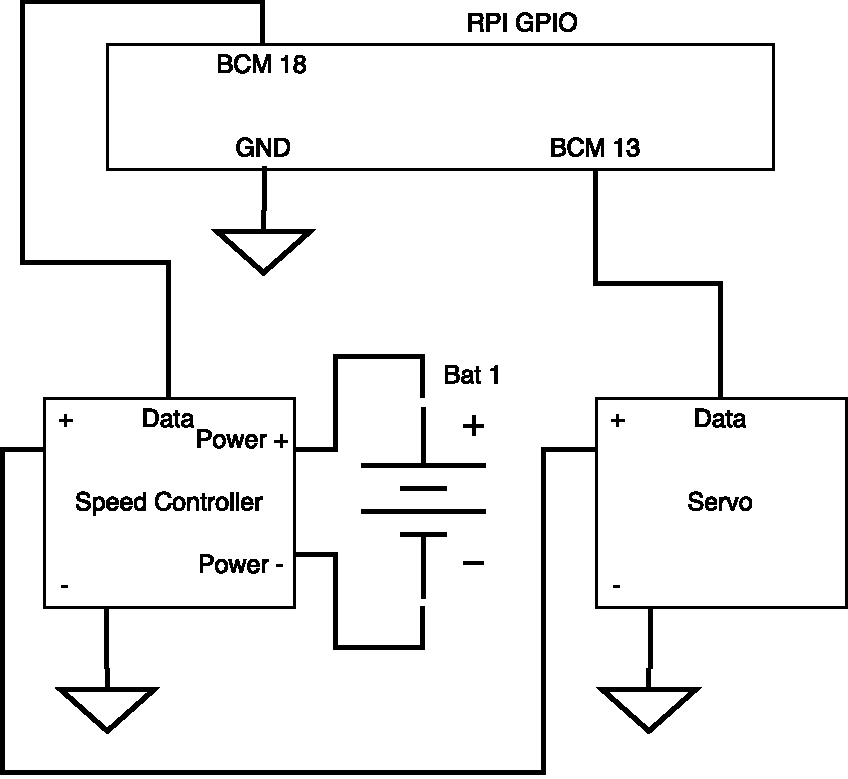
\includegraphics [scale =0.7] {figures/GPIODiagram.pdf}
\end{figure}

\begin{figure} [h!]
	\caption{Circuit Diagram - Raspberry Pi Power Supply}
	\centering
	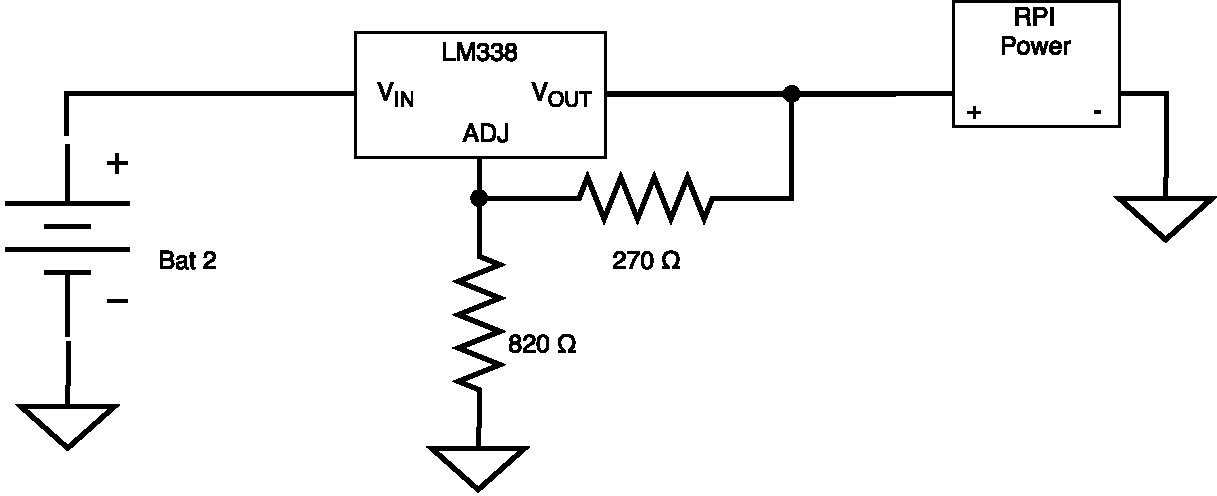
\includegraphics [scale =0.7] {figures/PowerDiagram.pdf}
\end{figure}

\break

\newpage



\section{ImageData Reference} \label{ImageData Reference}
The following figure provides an example of the image captured and processed by the ImageProcessing module. This will allows us to transform this image into useful data for the ImageData struct.

The blue horizontal line at the top represents the cutoff point for the image, anything above this line is ignored.\\
The blue circle at the bottom of the image represents the center point of the car. \\
The yellow circle represents the trajectory point. A desired point the car should attempt to reach. \\
The green lines to the left of the center point provide a means to calculate the average left angle, and the average left line length. Likewise for the green lines to the right of the center point, allows us to calculate the average right angle, and average right line length. \\

The white lines were captured through OpenCV's Canny Edge Detector algorithm, and the red lines were processed through OpenCV's Hough Transform for detecting straight lines.

\begin{figure} [h!]
	\caption{Image Information set by the Image Processing Module}
	\centering
	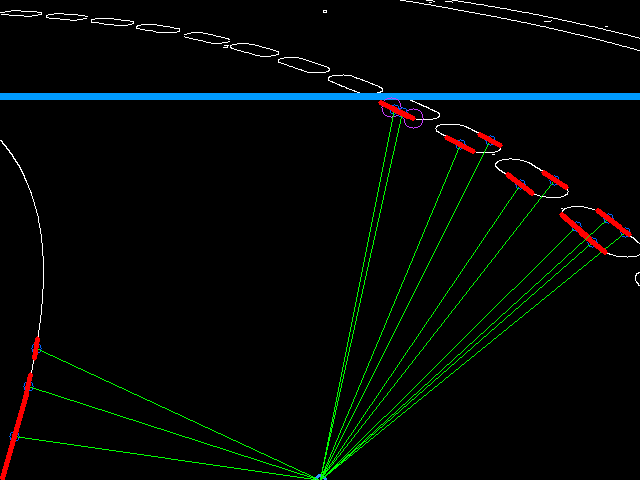
\includegraphics [scale=0.8] {figures/left_h.png}
	\label{fig:ImageData Example}
\end{figure}







\section{Scheduling}

\newpage
\pagestyle{fancy}

\paperwidth=\pdfpageheight
\paperheight=\pdfpagewidth
\pdfpageheight=\paperheight
\pdfpagewidth=\paperwidth
\headwidth=\textheight


\begingroup

%% 
\vsize=\textwidth
\hsize=\textheight



\break
\begin {figure}[h!]
\centering
\caption{Intersection Component Sequence Diagram} \vspace{4mm} \hspace*{-2cm}
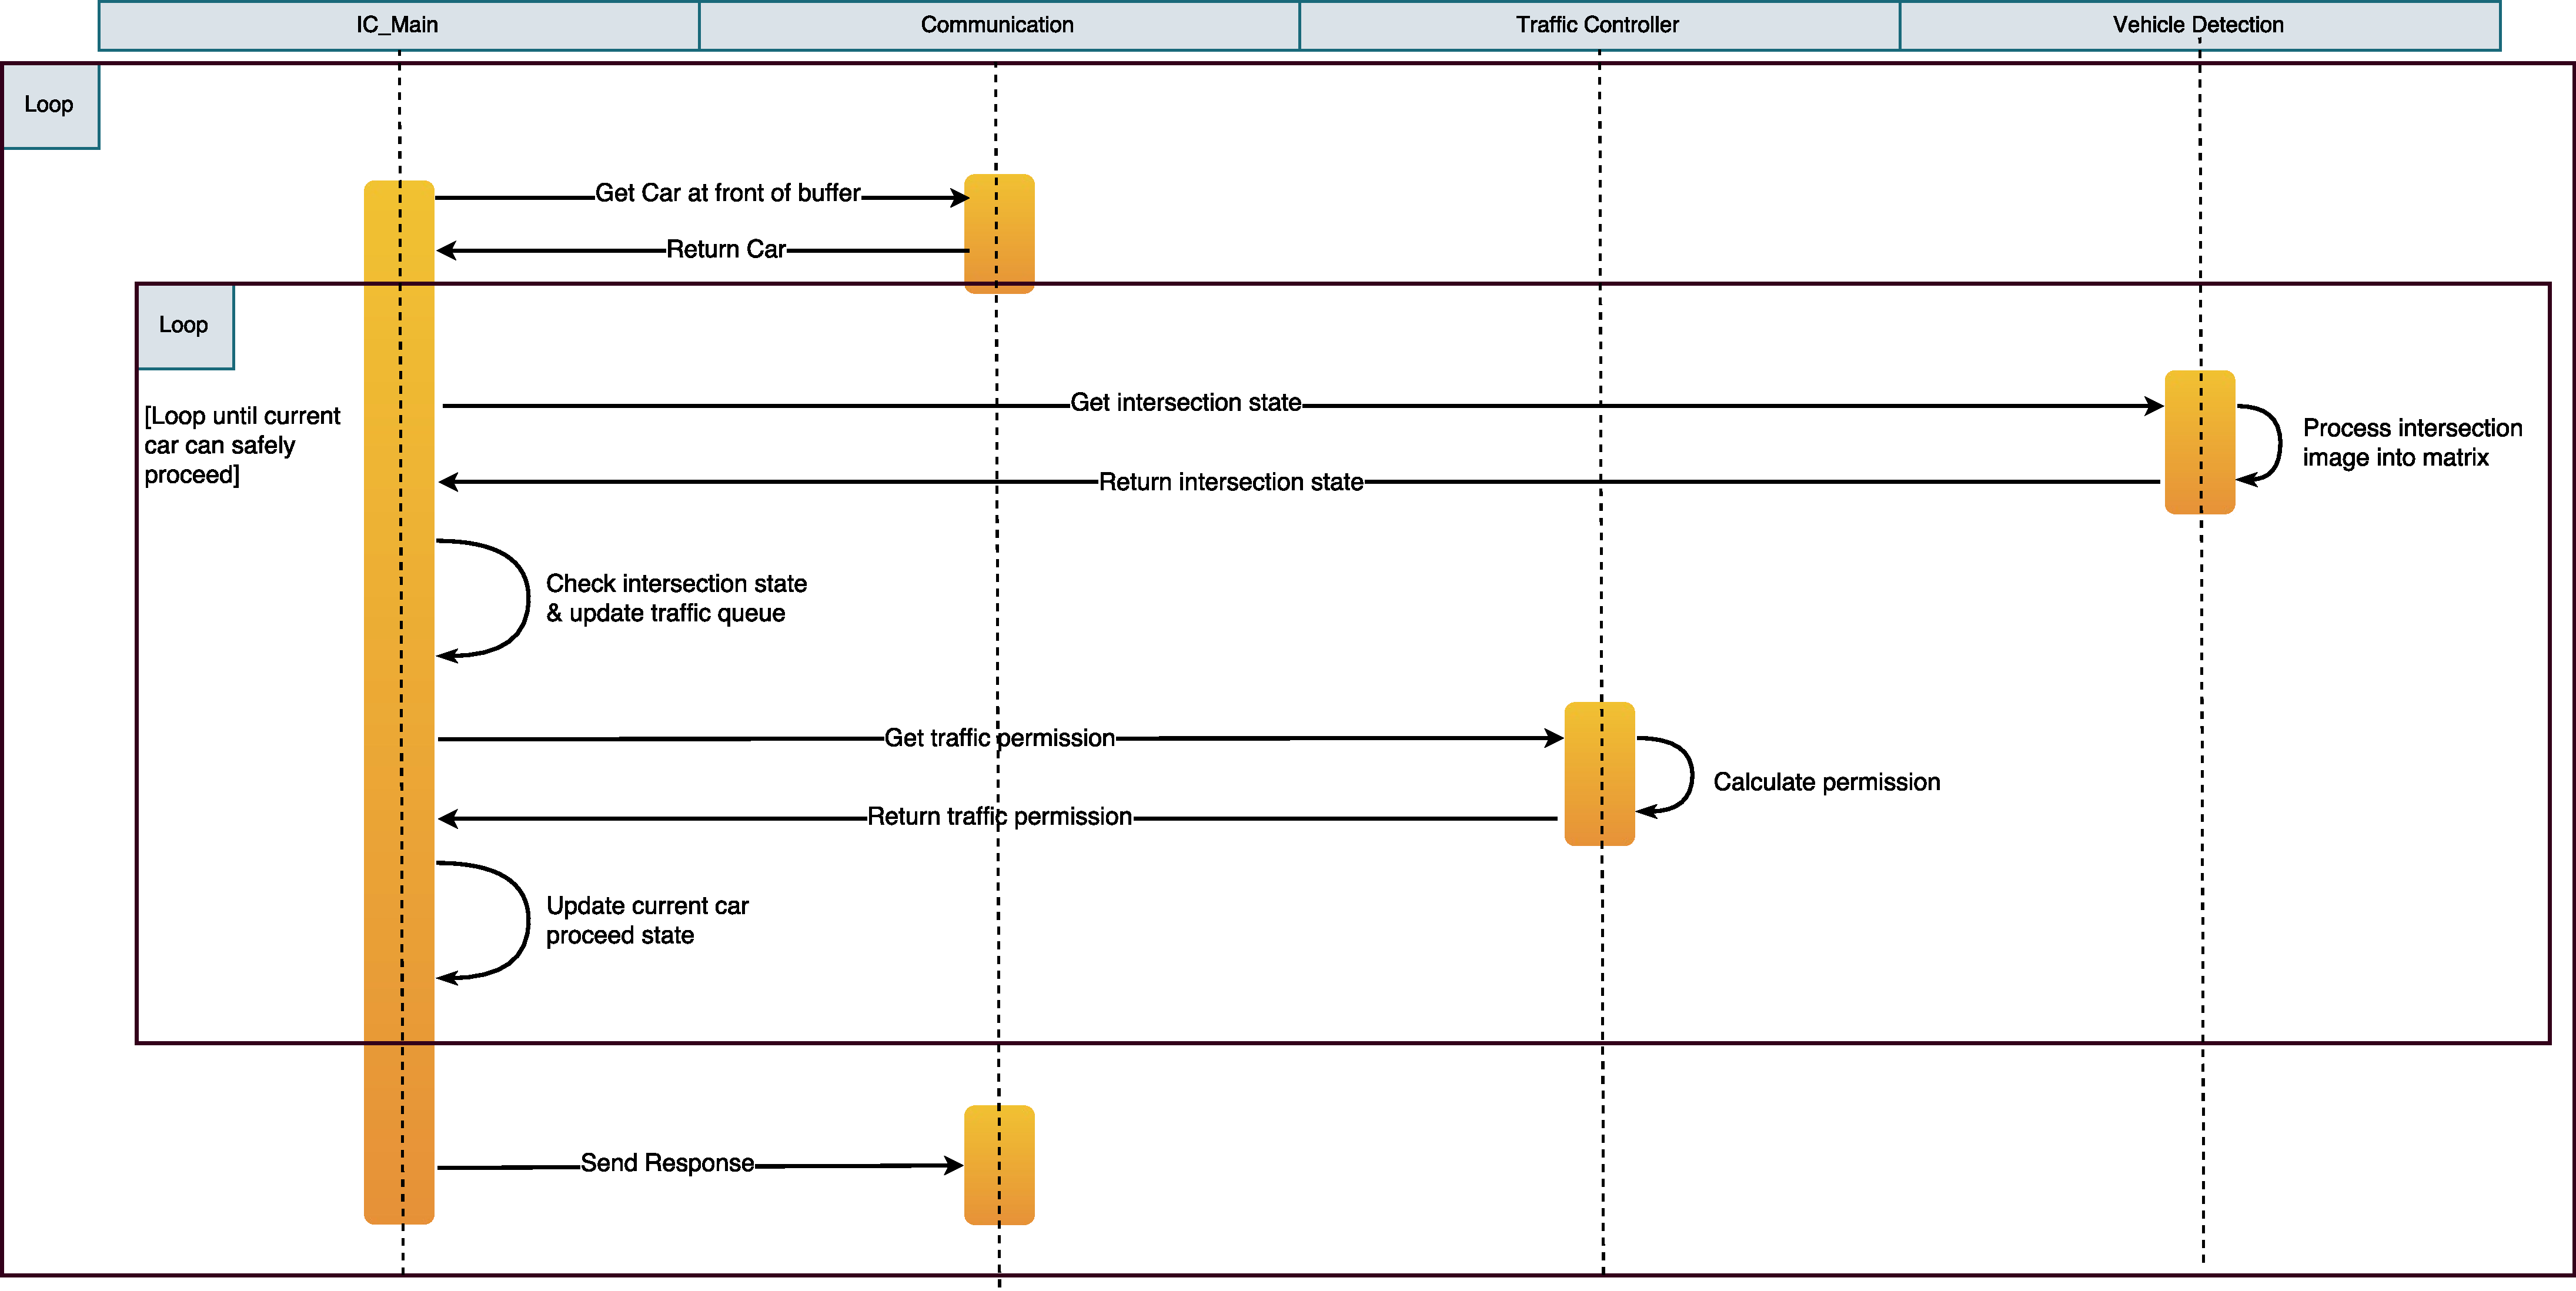
\includegraphics [scale = .36, angle = 0, trim={0 0 0 0},clip] {figures/IC_Sequence_Diagram.pdf}

\end{figure}



% This adds the pagenumber to the rotated page
\begin{landscape}
\end{landscape}
\endgroup


% This resets geometry after the landscape page
\newpage
\paperwidth=\pdfpageheight
\paperheight=\pdfpagewidth
\pdfpageheight=\paperheight
\pdfpagewidth=\paperwidth
\headwidth=\textwidth


\begin {figure}[h!]
\centering
\caption{Vehicle Component Sequence Diagram} \vspace{4mm}
\hspace*{-1.4cm}
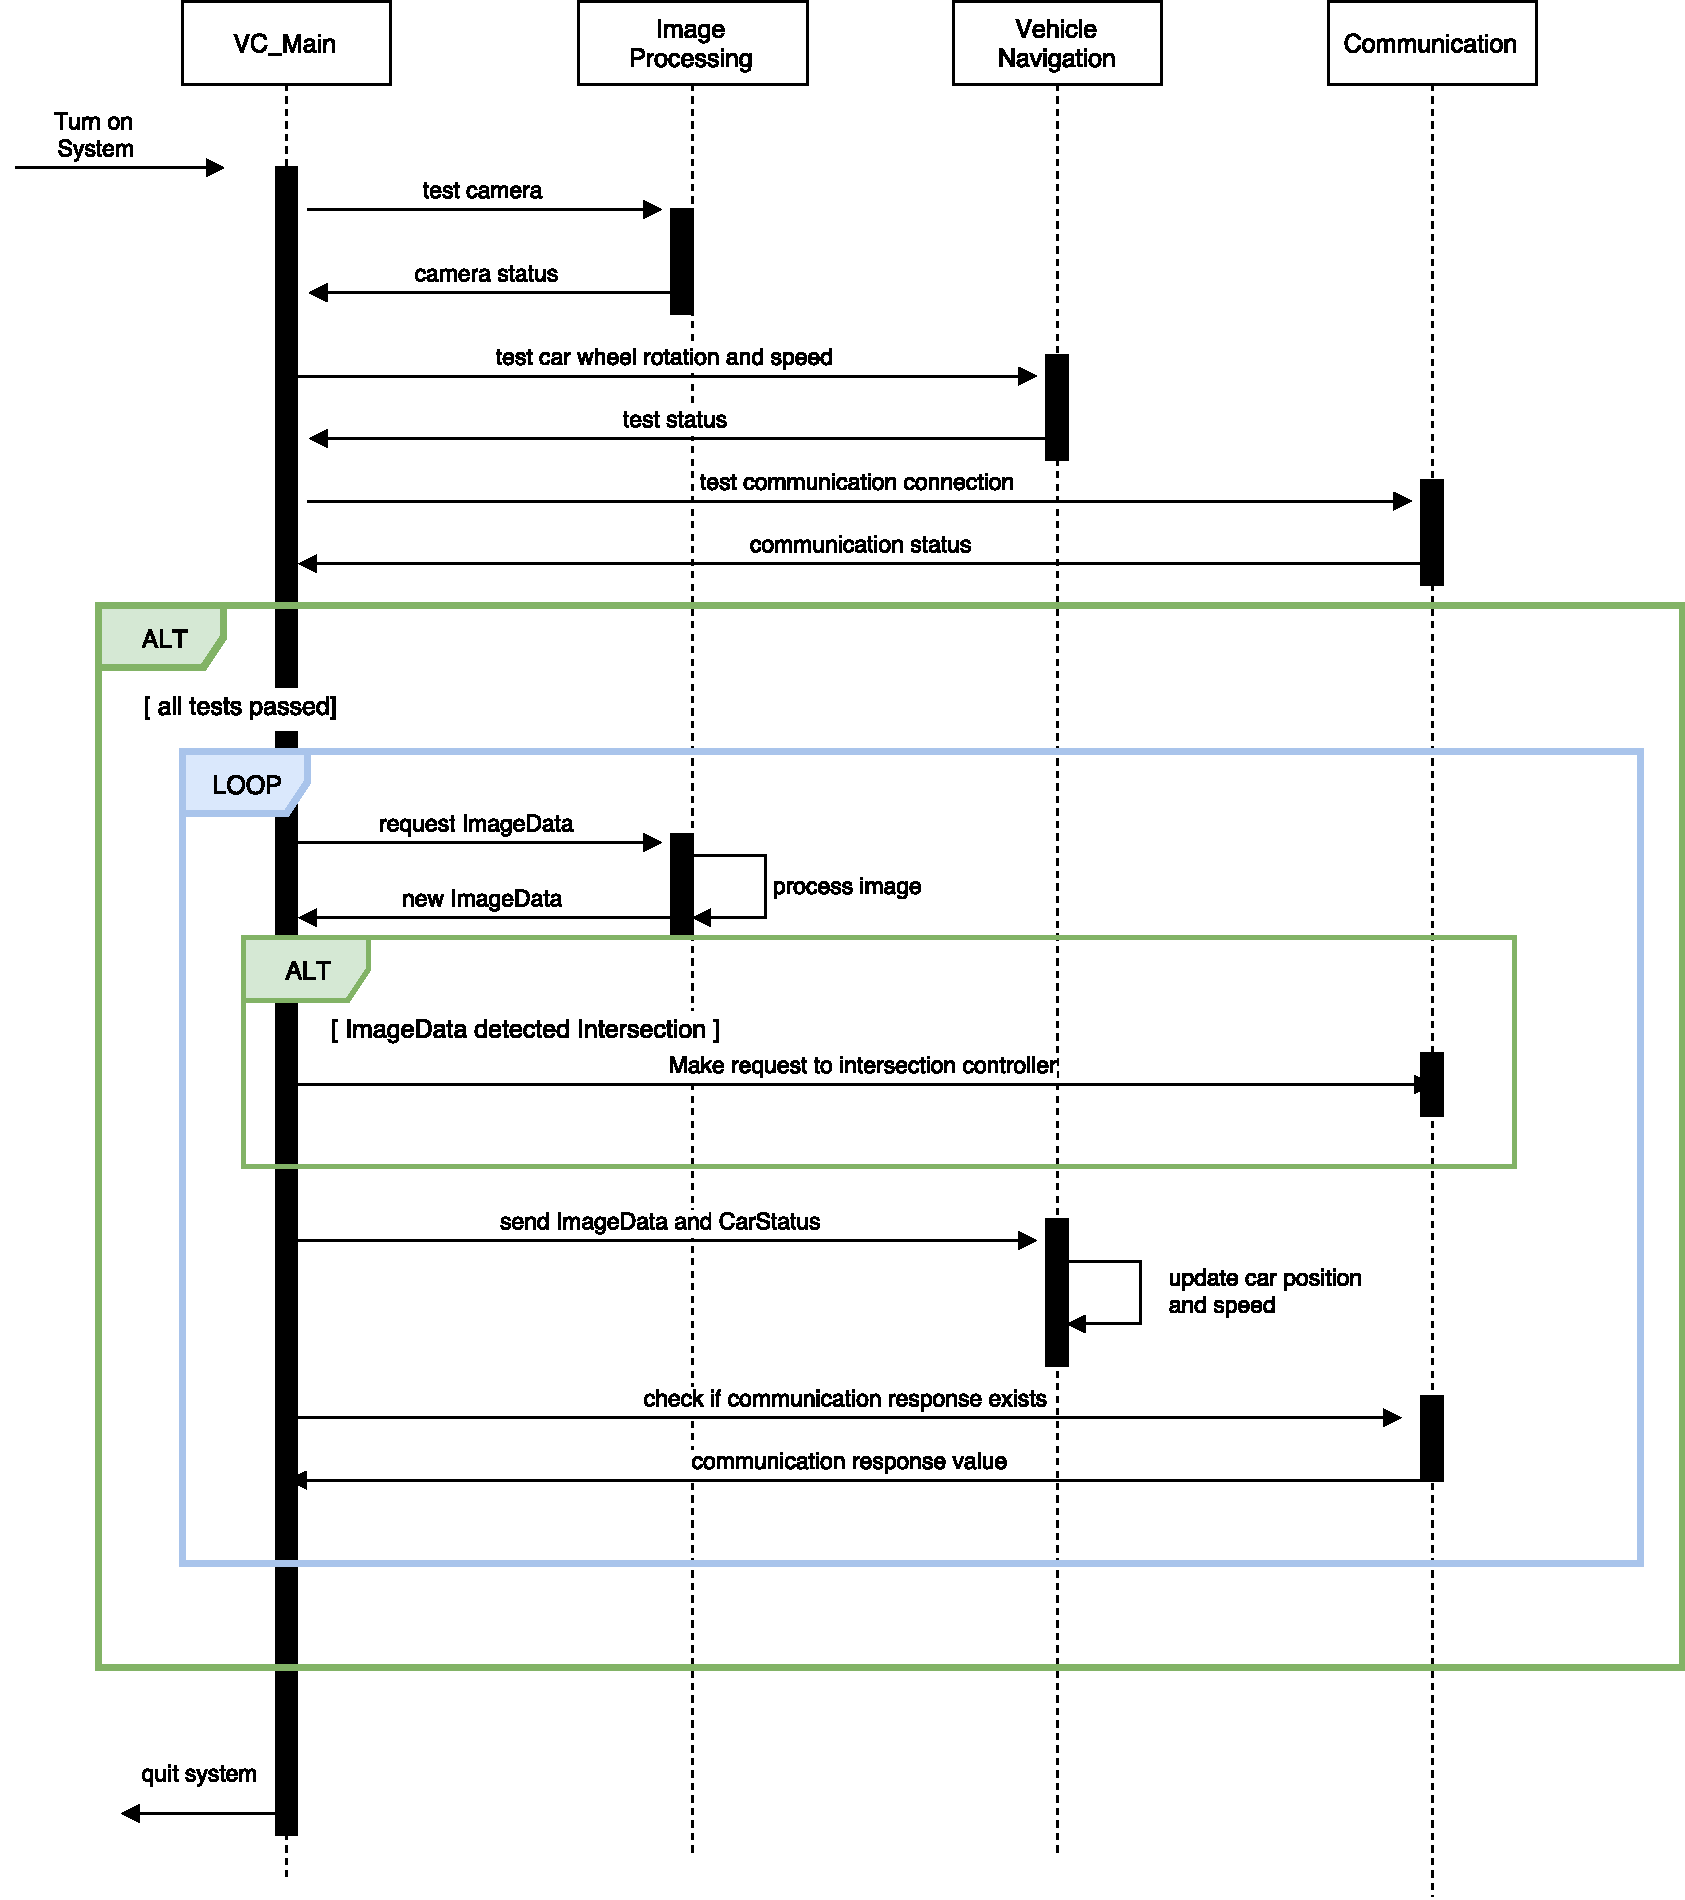
\includegraphics [scale = .68, trim={0 0 0 0},clip] {figures/carSequenceDiag.pdf}

\end {figure}






\end{document}
